\chapter{Pandas}

\section{¿Qué es Pandas?}

Pandas es una biblioteca de Python y sirve para analizar datos. Tiene
funciones para analizar, limpiar, explorar y manipular datos.

Pandas es una herramienta de análisis y manipulación de datos de código
abierto rápida, potente, flexible y fácil de usar, construida sobre el
lenguaje de programación Python.

El nombre "Pandas" hace referencia tanto a "Panel Data" como a "Python
Data Analysis" y fue creado por Wes McKinney en 2008.

El código fuente de Pandas se encuentra en un
\href{https://github.com/pandas-dev/pandas}{repositorio de GitHub}.

\section{Historia de su desarrollo}

En 2008, AQR Capital Management comenzó a desarrollar pandas. A fines de
2009, ya era de código abierto y, en la actualidad, cuenta con el apoyo
activo de una comunidad de personas con ideas afines en todo el mundo
que contribuyen con su valioso tiempo y energía para ayudar a que el
código abierto de pandas sea posible. Gracias a todos nuestros
colaboradores.

Desde 2015, pandas es un
\href{https://numfocus.org/sponsored-projects}{proyecto patrocinado por
NumFOCUS}. Esto ayudará a garantizar el éxito del desarrollo de pandas
como un proyecto de código abierto de clase mundial.

\section{Documentación}

Pandas posee una muy buena documentación en su
\href{https://pandas.pydata.org/docs/}{sitio web oficial}. En ella se
puede encontrar una guía rápida de uso, además de la documentación
completa del paquete.

\section{¿Porqué usar Pandas?}

Pandas nos permite analizar grandes cantidades de datos y sacar
conclusiones basadas en teorías estadísticas.

Pandas puede limpiar conjuntos de datos desordenados y hacerlos legibles
y relevantes.

Los datos relevantes son muy importantes en la ciencia de datos.

Pandas puede dar respuestas sobre los datos. Por ejemplo:

\begin{itemize}
  \item ¿Existe una correlación entre dos o más columnas?
  \item ¿Qué es el valor promedio?
  \item ¿Valor máximo?
  \item ¿Valor mínimo?
\end{itemize}

Pandas también puede eliminar filas que no son relevantes o que
contienen valores incorrectos, como valores vacíos o NULL. Esto se llama
limpiar los datos.

\section{Instalación} 
Si ya tiene Python y PIP instalados en un sistema, entonces la
instalación de Pandas es muy sencilla. Instálelo usando este comando:

\begin{Shaded}
\begin{Highlighting}[]
\ExtensionTok{$}\NormalTok{ pip install pandas}
\end{Highlighting}
\end{Shaded}

Si este comando falla, entonces use una distribución de Python que ya
tenga Pandas instalado, como Anaconda, Spyder, etc.

\section{Importar Pandas}

Una vez que Pandas esté instalado, impórtelo en sus aplicaciones
agregando la palabra clave \texttt{import}:

\begin{Shaded}
\begin{Highlighting}[]
\ImportTok{import}\NormalTok{ pandas}
\end{Highlighting}
\end{Shaded}

Con esto Pandas está importado y listo para usarse. \\

\begin{code} Creación de un DataFrame.

\begin{Shaded}
\begin{Highlighting}[]
\ImportTok{import}\NormalTok{ pandas}

\NormalTok{mydataset }\OperatorTok{=}\NormalTok{ \{}
  \StringTok{\textquotesingle{}cars\textquotesingle{}}\NormalTok{: [}\StringTok{"BMW"}\NormalTok{, }\StringTok{"Volvo"}\NormalTok{, }\StringTok{"Ford"}\NormalTok{],}
  \StringTok{\textquotesingle{}passings\textquotesingle{}}\NormalTok{: [}\DecValTok{3}\NormalTok{, }\DecValTok{7}\NormalTok{, }\DecValTok{2}\NormalTok{]}
\NormalTok{\}}

\NormalTok{myvar }\OperatorTok{=}\NormalTok{ pandas.DataFrame(mydataset)}

\BuiltInTok{print}\NormalTok{(myvar)}
\end{Highlighting}
\end{Shaded}

\begin{verbatim}
    cars  passings
0    BMW         3
1  Volvo         7
2   Ford         2
\end{verbatim}
\end{code}

Al importar pandas se puede emplear el alias \texttt{pd}. Ahora, el
paquete Pandas se puede invocar con \texttt{pd} en lugar del nombre
completo \texttt{pandas}.\\

\begin{code} Creación de un alias para un DataFrame.
\begin{Shaded}
\begin{Highlighting}[]
\ImportTok{import}\NormalTok{ pandas }\ImportTok{as}\NormalTok{ pd}

\NormalTok{mydataset }\OperatorTok{=}\NormalTok{ \{}
  \StringTok{\textquotesingle{}cars\textquotesingle{}}\NormalTok{: [}\StringTok{"BMW"}\NormalTok{, }\StringTok{"Volvo"}\NormalTok{, }\StringTok{"Ford"}\NormalTok{],}
  \StringTok{\textquotesingle{}passings\textquotesingle{}}\NormalTok{: [}\DecValTok{3}\NormalTok{, }\DecValTok{7}\NormalTok{, }\DecValTok{2}\NormalTok{]}
\NormalTok{\}}

\NormalTok{myvar }\OperatorTok{=}\NormalTok{ pd.DataFrame(mydataset)}

\BuiltInTok{print}\NormalTok{(myvar)}
\end{Highlighting}
\end{Shaded}

\begin{verbatim}
    cars  passings
0    BMW         3
1  Volvo         7
2   Ford         2
\end{verbatim}
\end{code}

\section{Verificando la versión}

La versión de pandas se almacena en una cadena almacenada en el atributo \texttt{\_\_version\_\_}.

\begin{code} Verificación de la versión de \texttt{pandas}.
\begin{Shaded}
\begin{Highlighting}[]
\ImportTok{import}\NormalTok{ pandas }\ImportTok{as}\NormalTok{ pd}

\BuiltInTok{print}\NormalTok{(pd.\_\_version\_\_)}
\end{Highlighting}
\end{Shaded}

\begin{verbatim}
2.2.2
\end{verbatim}
\end{code}

\section{Series Pandas}

Una serie de Pandas es como una columna de una tabla. Es una matriz unidimensional que contiene datos de cualquier tipo.\\

\begin{code} Crear una serie de pandas a partir de una lista.

\begin{Shaded}
\begin{Highlighting}[]
\ImportTok{import}\NormalTok{ pandas }\ImportTok{as}\NormalTok{ pd}

\NormalTok{a }\OperatorTok{=}\NormalTok{ [}\DecValTok{1}\NormalTok{, }\DecValTok{7}\NormalTok{, }\DecValTok{2}\NormalTok{]}

\NormalTok{myvar }\OperatorTok{=}\NormalTok{ pd.Series(a)}

\BuiltInTok{print}\NormalTok{(myvar)}
\end{Highlighting}
\end{Shaded}

\begin{verbatim}
0    1
1    7
2    2
dtype: int64
\end{verbatim}
\end{code}

Si no se especifica nada más, los valores se etiquetan con su número de
índice. El primer valor tiene el índice 0, el segundo valor tiene el
índice 1, etc.

Esta etiqueta se puede utilizar para acceder a un valor especifico.\\

\begin{code} Devolver el primer valor de la serie.

\begin{Shaded}
\begin{Highlighting}[]
\BuiltInTok{print}\NormalTok{(myvar[}\DecValTok{0}\NormalTok{])}
\end{Highlighting}
\end{Shaded}

\begin{verbatim}
1
\end{verbatim}
\end{code}

Con el argumento \texttt{index} se puede nombrar las etiquetas.\\

\begin{code} Crear etiquetas propias.

\begin{Shaded}
\begin{Highlighting}[]
\ImportTok{import}\NormalTok{ pandas }\ImportTok{as}\NormalTok{ pd}

\NormalTok{a }\OperatorTok{=}\NormalTok{ [}\DecValTok{1}\NormalTok{, }\DecValTok{7}\NormalTok{, }\DecValTok{2}\NormalTok{]}

\NormalTok{myvar }\OperatorTok{=}\NormalTok{ pd.Series(a, index }\OperatorTok{=}\NormalTok{ [}\StringTok{"x"}\NormalTok{, }\StringTok{"y"}\NormalTok{, }\StringTok{"z"}\NormalTok{])}

\BuiltInTok{print}\NormalTok{(myvar)}
\end{Highlighting}
\end{Shaded}

\begin{verbatim}
x    1
y    7
z    2
dtype: int64
\end{verbatim}
\end{code}

Una vez que haya creado etiquetas, podrá acceder a un elemento haciendo referencia a la etiqueta.\\

\begin{code} Devolver el valor de ``y''.

\begin{Shaded}
\begin{Highlighting}[]
\BuiltInTok{print}\NormalTok{(myvar[}\StringTok{"y"}\NormalTok{])}
\end{Highlighting}
\end{Shaded}

\begin{verbatim}
7
\end{verbatim}
\end{code}

\section{Objetos llave/valor como series}

También puedes utilizar un objeto clave/valor, como un diccionario, al crear una Serie.\\

\begin{code} Crea una serie Pandas sencilla a partir de un diccionario.

\begin{Shaded}
\begin{Highlighting}[]
\ImportTok{import}\NormalTok{ pandas }\ImportTok{as}\NormalTok{ pd}

\NormalTok{calories }\OperatorTok{=}\NormalTok{ \{}\StringTok{"day1"}\NormalTok{: }\DecValTok{420}\NormalTok{, }\StringTok{"day2"}\NormalTok{: }\DecValTok{380}\NormalTok{, }\StringTok{"day3"}\NormalTok{: }\DecValTok{390}\NormalTok{\}}

\NormalTok{myvar }\OperatorTok{=}\NormalTok{ pd.Series(calories)}

\BuiltInTok{print}\NormalTok{(myvar)}
\end{Highlighting}
\end{Shaded}

\begin{verbatim}
day1    420
day2    380
day3    390
dtype: int64
\end{verbatim}
\end{code}

Observe que las claves del diccionario se convierten en las etiquetas.

Para seleccionar solo algunos de los elementos del diccionario, utilice
el argumento de índice y especifique solo los elementos que desea
incluir en la serie. \\

\begin{code} Cree una serie utilizando solo datos de ``día1'' y ``día2''.

\begin{Shaded}
\begin{Highlighting}[]
\ImportTok{import}\NormalTok{ pandas }\ImportTok{as}\NormalTok{ pd}

\NormalTok{calories }\OperatorTok{=}\NormalTok{ \{}\StringTok{"day1"}\NormalTok{: }\DecValTok{420}\NormalTok{, }\StringTok{"day2"}\NormalTok{: }\DecValTok{380}\NormalTok{, }\StringTok{"day3"}\NormalTok{: }\DecValTok{390}\NormalTok{\}}

\NormalTok{myvar }\OperatorTok{=}\NormalTok{ pd.Series(calories, index }\OperatorTok{=}\NormalTok{ [}\StringTok{"day1"}\NormalTok{, }\StringTok{"day2"}\NormalTok{])}

\BuiltInTok{print}\NormalTok{(myvar)}
\end{Highlighting}
\end{Shaded}

\begin{verbatim}
day1    420
day2    380
dtype: int64
\end{verbatim}
\end{code}

\section{DataFrames}

Los conjuntos de datos en Pandas suelen ser tablas multidimensionales, llamadas DataFrames.

Una serie es como una columna, un DataFrame es la tabla completa. \\

\begin{code} Crear un DataFrame a partir de dos series.

\begin{Shaded}
\begin{Highlighting}[]
\ImportTok{import}\NormalTok{ pandas }\ImportTok{as}\NormalTok{ pd}

\CommentTok{\# Diccionario data}
\NormalTok{data }\OperatorTok{=}\NormalTok{ \{}
  \StringTok{"calories"}\NormalTok{: [}\DecValTok{420}\NormalTok{, }\DecValTok{380}\NormalTok{, }\DecValTok{390}\NormalTok{],}
  \StringTok{"duration"}\NormalTok{: [}\DecValTok{50}\NormalTok{, }\DecValTok{40}\NormalTok{, }\DecValTok{45}\NormalTok{]}
\NormalTok{\}}

\NormalTok{df }\OperatorTok{=}\NormalTok{ pd.DataFrame(data)}

\BuiltInTok{print}\NormalTok{(df)}
\end{Highlighting}
\end{Shaded}

\begin{verbatim}
   calories  duration
0       420        50
1       380        40
2       390        45
\end{verbatim}
\end{code}

\subsection{¿Qué es un DataFrame?}

Un Pandas DataFrame es una estructura de datos de 2 dimensiones, como
una de 2 dimensiones array, o una tabla con filas y columnas.

Como puede ver en el resultado anterior, el DataFrame es como una tabla
con filas y columnas.

\subsection{Localizar una fila}

Los pandas usan el atributo \texttt{loc} a devolver una o más filas
especificadas. \\

\begin{code} Devolver la fila 0.

\begin{Shaded}
\begin{Highlighting}[]
\BuiltInTok{print}\NormalTok{(df.loc[}\DecValTok{0}\NormalTok{])}
\end{Highlighting}
\end{Shaded}

\begin{verbatim}
calories    420
duration     50
Name: 0, dtype: int64
\end{verbatim}
\end{code}

Este código devuelve una serie Pandas.\\

\begin{code} Devolver filas 0 y 1.

\begin{Shaded}
\begin{Highlighting}[]
\BuiltInTok{print}\NormalTok{(df.loc[[}\DecValTok{0}\NormalTok{, }\DecValTok{1}\NormalTok{]])}
\end{Highlighting}
\end{Shaded}

\begin{verbatim}
   calories  duration
0       420        50
1       380        40
\end{verbatim}
\end{code}

En este caso, el código devuelve un DataFrame Pandas.

\subsection{Índices nombrados}

Con el argumento \texttt{index}, se puede nombrar sus propios índices.
Nótese que los índices deben ser una lista.\\

\begin{code} DataFrame con índices nombrados.

\begin{Shaded}
\begin{Highlighting}[]
\ImportTok{import}\NormalTok{ pandas }\ImportTok{as}\NormalTok{ pd}

\NormalTok{data }\OperatorTok{=}\NormalTok{ \{}
  \StringTok{"calories"}\NormalTok{: [}\DecValTok{420}\NormalTok{, }\DecValTok{380}\NormalTok{, }\DecValTok{390}\NormalTok{],}
  \StringTok{"duration"}\NormalTok{: [}\DecValTok{50}\NormalTok{, }\DecValTok{40}\NormalTok{, }\DecValTok{45}\NormalTok{]}
\NormalTok{\}}

\NormalTok{df }\OperatorTok{=}\NormalTok{ pd.DataFrame(data, index }\OperatorTok{=}\NormalTok{ [}\StringTok{"day1"}\NormalTok{, }\StringTok{"day2"}\NormalTok{, }\StringTok{"day3"}\NormalTok{])}

\BuiltInTok{print}\NormalTok{(df) }
\end{Highlighting}
\end{Shaded}

\begin{verbatim}
      calories  duration
day1       420        50
day2       380        40
day3       390        45
\end{verbatim}
\end{code}

\subsection{Localizar Índices Nombrados}

Utilice el índice nombrado en el atributo \texttt{loc} para devolver la fila especificada.\\

\begin{code} Retorno ``day2''.

\begin{Shaded}
\begin{Highlighting}[]
\CommentTok{\# Referencia al índice nombrado:}
\BuiltInTok{print}\NormalTok{(df.loc[}\StringTok{"day2"}\NormalTok{])}
\end{Highlighting}
\end{Shaded}

\begin{verbatim}
calories    380
duration     40
Name: day2, dtype: int64
\end{verbatim}
\end{code}

\subsection{Carga de archivos en un DataFrame}

Una forma sencilla de almacenar grandes conjuntos de datos es usar
archivos CSV (separados por comas archivos).

Los archivos CSV contienen texto sin formato y es un formato bien
conocido que puede ser leído por todos, incluyendo Pandas.

Si sus conjuntos de datos se almacenan en un archivo, Pandas puede
cargarlos en un DataFrame.\\

\begin{code} Cargue un archivo separado por comas (Archivo CSV) en un DataFrame.

\begin{Shaded}
\begin{Highlighting}[]
\ImportTok{import}\NormalTok{ pandas }\ImportTok{as}\NormalTok{ pd}

\NormalTok{df }\OperatorTok{=}\NormalTok{ pd.read\_csv(}\StringTok{\textquotesingle{}data/data.csv\textquotesingle{}}\NormalTok{)}

\BuiltInTok{print}\NormalTok{(df) }
\end{Highlighting}
\end{Shaded}

\begin{verbatim}
     Duration  Pulse  Maxpulse  Calories
0          60    110       130     409.1
1          60    117       145     479.0
2          60    103       135     340.0
3          45    109       175     282.4
4          45    117       148     406.0
..        ...    ...       ...       ...
164        60    105       140     290.8
165        60    110       145     300.0
166        60    115       145     310.2
167        75    120       150     320.4
168        75    125       150     330.4

[169 rows x 4 columns]
\end{verbatim}
\end{code}

Si tiene un DataFrame grande con muchas filas, Pandas solo devolverá las
primeras 5 filas y las últimas 5 filas.

Se puede emplear el método \texttt{to\_string()} para convertir el
DataFrame en una sola representación String. La salida es una tabla
amigable para la consola.\\

\begin{code} Método \texttt{to\_string()} para convertir el DataFrame en una sola representación String.
\begin{Shaded}
\begin{Highlighting}[]
\ImportTok{import}\NormalTok{ pandas }\ImportTok{as}\NormalTok{ pd}

\NormalTok{df }\OperatorTok{=}\NormalTok{ pd.read\_csv(}\StringTok{\textquotesingle{}data/data.csv\textquotesingle{}}\NormalTok{)}

\BuiltInTok{print}\NormalTok{(df.to\_string()) }
\end{Highlighting}
\end{Shaded}

\begin{verbatim}
     Duration  Pulse  Maxpulse  Calories
0          60    110       130     409.1
1          60    117       145     479.0
2          60    103       135     340.0
3          45    109       175     282.4
4          45    117       148     406.0
5          60    102       127     300.0
6          60    110       136     374.0
7          45    104       134     253.3
8          30    109       133     195.1
9          60     98       124     269.0
10         60    103       147     329.3
11         60    100       120     250.7
12         60    106       128     345.3
13         60    104       132     379.3
14         60     98       123     275.0
15         60     98       120     215.2
16         60    100       120     300.0
17         45     90       112       NaN
18         60    103       123     323.0
19         45     97       125     243.0
20         60    108       131     364.2
21         45    100       119     282.0
22         60    130       101     300.0
23         45    105       132     246.0
24         60    102       126     334.5
25         60    100       120     250.0
26         60     92       118     241.0
27         60    103       132       NaN
28         60    100       132     280.0
29         60    102       129     380.3
30         60     92       115     243.0
31         45     90       112     180.1
32         60    101       124     299.0
33         60     93       113     223.0
34         60    107       136     361.0
35         60    114       140     415.0
36         60    102       127     300.0
37         60    100       120     300.0
38         60    100       120     300.0
39         45    104       129     266.0
40         45     90       112     180.1
41         60     98       126     286.0
42         60    100       122     329.4
43         60    111       138     400.0
44         60    111       131     397.0
45         60     99       119     273.0
46         60    109       153     387.6
47         45    111       136     300.0
48         45    108       129     298.0
49         60    111       139     397.6
50         60    107       136     380.2
51         80    123       146     643.1
52         60    106       130     263.0
53         60    118       151     486.0
54         30    136       175     238.0
55         60    121       146     450.7
56         60    118       121     413.0
57         45    115       144     305.0
58         20    153       172     226.4
59         45    123       152     321.0
60        210    108       160    1376.0
61        160    110       137    1034.4
62        160    109       135     853.0
63         45    118       141     341.0
64         20    110       130     131.4
65        180     90       130     800.4
66        150    105       135     873.4
67        150    107       130     816.0
68         20    106       136     110.4
69        300    108       143    1500.2
70        150     97       129    1115.0
71         60    109       153     387.6
72         90    100       127     700.0
73        150     97       127     953.2
74         45    114       146     304.0
75         90     98       125     563.2
76         45    105       134     251.0
77         45    110       141     300.0
78        120    100       130     500.4
79        270    100       131    1729.0
80         30    159       182     319.2
81         45    149       169     344.0
82         30    103       139     151.1
83        120    100       130     500.0
84         45    100       120     225.3
85         30    151       170     300.0
86         45    102       136     234.0
87        120    100       157    1000.1
88         45    129       103     242.0
89         20     83       107      50.3
90        180    101       127     600.1
91         45    107       137       NaN
92         30     90       107     105.3
93         15     80       100      50.5
94         20    150       171     127.4
95         20    151       168     229.4
96         30     95       128     128.2
97         25    152       168     244.2
98         30    109       131     188.2
99         90     93       124     604.1
100        20     95       112      77.7
101        90     90       110     500.0
102        90     90       100     500.0
103        90     90       100     500.4
104        30     92       108      92.7
105        30     93       128     124.0
106       180     90       120     800.3
107        30     90       120      86.2
108        90     90       120     500.3
109       210    137       184    1860.4
110        60    102       124     325.2
111        45    107       124     275.0
112        15    124       139     124.2
113        45    100       120     225.3
114        60    108       131     367.6
115        60    108       151     351.7
116        60    116       141     443.0
117        60     97       122     277.4
118        60    105       125       NaN
119        60    103       124     332.7
120        30    112       137     193.9
121        45    100       120     100.7
122        60    119       169     336.7
123        60    107       127     344.9
124        60    111       151     368.5
125        60     98       122     271.0
126        60     97       124     275.3
127        60    109       127     382.0
128        90     99       125     466.4
129        60    114       151     384.0
130        60    104       134     342.5
131        60    107       138     357.5
132        60    103       133     335.0
133        60    106       132     327.5
134        60    103       136     339.0
135        20    136       156     189.0
136        45    117       143     317.7
137        45    115       137     318.0
138        45    113       138     308.0
139        20    141       162     222.4
140        60    108       135     390.0
141        60     97       127       NaN
142        45    100       120     250.4
143        45    122       149     335.4
144        60    136       170     470.2
145        45    106       126     270.8
146        60    107       136     400.0
147        60    112       146     361.9
148        30    103       127     185.0
149        60    110       150     409.4
150        60    106       134     343.0
151        60    109       129     353.2
152        60    109       138     374.0
153        30    150       167     275.8
154        60    105       128     328.0
155        60    111       151     368.5
156        60     97       131     270.4
157        60    100       120     270.4
158        60    114       150     382.8
159        30     80       120     240.9
160        30     85       120     250.4
161        45     90       130     260.4
162        45     95       130     270.0
163        45    100       140     280.9
164        60    105       140     290.8
165        60    110       145     300.0
166        60    115       145     310.2
167        75    120       150     320.4
168        75    125       150     330.4

\end{verbatim}
\end{code}

\begin{code} Método \texttt{to\_string()} para convertir el DataFrame en una sola representación String.
\begin{Shaded}
\begin{Highlighting}[]
\ImportTok{import}\NormalTok{ pandas }\ImportTok{as}\NormalTok{ pd}

\NormalTok{df }\OperatorTok{=}\NormalTok{ pd.read\_csv(}\StringTok{\textquotesingle{}data/social.csv\textquotesingle{}}\NormalTok{)}

\BuiltInTok{print}\NormalTok{(df.to\_string()) }
\end{Highlighting}
\end{Shaded}

\begin{verbatim}
  Social media platform Number of monthly (million)
0              Facebook                      3 000m
1               YouTube                    2000.5 m
2             Instagram                      2 000m
3                TikTok                    1000.5 m
4              Snapchat                       800 m
5           X (Twitter)                       611 m
6                Reddit                       500 m
7             Pinterest                       498 m
8              LinkedIn                       350 m
9               Threads                       175 m
\end{verbatim}
\end{code}

\subsection{\texorpdfstring{\texttt{max\_filas}}{max\_filas}}

El número de filas devueltas se define en la configuración de la opción
Pandas. Puede verificar las filas máximas de su sistema con la
declaración \texttt{pd.options.display.max\_rows}.\\

\begin{code} Verificación del número máximo de filas.
\begin{Shaded}
\begin{Highlighting}[]
\ImportTok{import}\NormalTok{ pandas }\ImportTok{as}\NormalTok{ pd}

\BuiltInTok{print}\NormalTok{(pd.options.display.max\_rows) }
\end{Highlighting}
\end{Shaded}

\begin{verbatim}
60
\end{verbatim}
\end{code}

En mi sistema el número es 60, lo que significa que si el DataFrame
contiene más de 60 filas, el \texttt{print(df)} la declaración devolverá
solo los encabezados y las primeras y últimas 5 filas.

Puede cambiar el número máximo de filas con la misma instrucción.\\

\begin{code} Modificación del número máximo de filas.
\begin{Shaded}
\begin{Highlighting}[]
\ImportTok{import}\NormalTok{ pandas }\ImportTok{as}\NormalTok{ pd}

\NormalTok{pd.options.display.max\_rows }\OperatorTok{=} \DecValTok{9999}
\NormalTok{df }\OperatorTok{=}\NormalTok{ pd.read\_csv(}\StringTok{\textquotesingle{}data/data.csv\textquotesingle{}}\NormalTok{)}

\BuiltInTok{print}\NormalTok{(df) }
\end{Highlighting}
\end{Shaded}

\begin{verbatim}
     Duration  Pulse  Maxpulse  Calories
0          60    110       130     409.1
1          60    117       145     479.0
2          60    103       135     340.0
3          45    109       175     282.4
4          45    117       148     406.0
5          60    102       127     300.0
6          60    110       136     374.0
7          45    104       134     253.3
8          30    109       133     195.1
9          60     98       124     269.0
10         60    103       147     329.3
11         60    100       120     250.7
12         60    106       128     345.3
13         60    104       132     379.3
14         60     98       123     275.0
15         60     98       120     215.2
16         60    100       120     300.0
17         45     90       112       NaN
18         60    103       123     323.0
19         45     97       125     243.0
20         60    108       131     364.2
21         45    100       119     282.0
22         60    130       101     300.0
23         45    105       132     246.0
24         60    102       126     334.5
25         60    100       120     250.0
26         60     92       118     241.0
27         60    103       132       NaN
28         60    100       132     280.0
29         60    102       129     380.3
30         60     92       115     243.0
31         45     90       112     180.1
32         60    101       124     299.0
33         60     93       113     223.0
34         60    107       136     361.0
35         60    114       140     415.0
36         60    102       127     300.0
37         60    100       120     300.0
38         60    100       120     300.0
39         45    104       129     266.0
40         45     90       112     180.1
41         60     98       126     286.0
42         60    100       122     329.4
43         60    111       138     400.0
44         60    111       131     397.0
45         60     99       119     273.0
46         60    109       153     387.6
47         45    111       136     300.0
48         45    108       129     298.0
49         60    111       139     397.6
50         60    107       136     380.2
51         80    123       146     643.1
52         60    106       130     263.0
53         60    118       151     486.0
54         30    136       175     238.0
55         60    121       146     450.7
56         60    118       121     413.0
57         45    115       144     305.0
58         20    153       172     226.4
59         45    123       152     321.0
60        210    108       160    1376.0
61        160    110       137    1034.4
62        160    109       135     853.0
63         45    118       141     341.0
64         20    110       130     131.4
65        180     90       130     800.4
66        150    105       135     873.4
67        150    107       130     816.0
68         20    106       136     110.4
69        300    108       143    1500.2
70        150     97       129    1115.0
71         60    109       153     387.6
72         90    100       127     700.0
73        150     97       127     953.2
74         45    114       146     304.0
75         90     98       125     563.2
76         45    105       134     251.0
77         45    110       141     300.0
78        120    100       130     500.4
79        270    100       131    1729.0
80         30    159       182     319.2
81         45    149       169     344.0
82         30    103       139     151.1
83        120    100       130     500.0
84         45    100       120     225.3
85         30    151       170     300.0
86         45    102       136     234.0
87        120    100       157    1000.1
88         45    129       103     242.0
89         20     83       107      50.3
90        180    101       127     600.1
91         45    107       137       NaN
92         30     90       107     105.3
93         15     80       100      50.5
94         20    150       171     127.4
95         20    151       168     229.4
96         30     95       128     128.2
97         25    152       168     244.2
98         30    109       131     188.2
99         90     93       124     604.1
100        20     95       112      77.7
101        90     90       110     500.0
102        90     90       100     500.0
103        90     90       100     500.4
104        30     92       108      92.7
105        30     93       128     124.0
106       180     90       120     800.3
107        30     90       120      86.2
108        90     90       120     500.3
109       210    137       184    1860.4
110        60    102       124     325.2
111        45    107       124     275.0
112        15    124       139     124.2
113        45    100       120     225.3
114        60    108       131     367.6
115        60    108       151     351.7
116        60    116       141     443.0
117        60     97       122     277.4
118        60    105       125       NaN
119        60    103       124     332.7
120        30    112       137     193.9
121        45    100       120     100.7
122        60    119       169     336.7
123        60    107       127     344.9
124        60    111       151     368.5
125        60     98       122     271.0
126        60     97       124     275.3
127        60    109       127     382.0
128        90     99       125     466.4
129        60    114       151     384.0
130        60    104       134     342.5
131        60    107       138     357.5
132        60    103       133     335.0
133        60    106       132     327.5
134        60    103       136     339.0
135        20    136       156     189.0
136        45    117       143     317.7
137        45    115       137     318.0
138        45    113       138     308.0
139        20    141       162     222.4
140        60    108       135     390.0
141        60     97       127       NaN
142        45    100       120     250.4
143        45    122       149     335.4
144        60    136       170     470.2
145        45    106       126     270.8
146        60    107       136     400.0
147        60    112       146     361.9
148        30    103       127     185.0
149        60    110       150     409.4
150        60    106       134     343.0
151        60    109       129     353.2
152        60    109       138     374.0
153        30    150       167     275.8
154        60    105       128     328.0
155        60    111       151     368.5
156        60     97       131     270.4
157        60    100       120     270.4
158        60    114       150     382.8
159        30     80       120     240.9
160        30     85       120     250.4
161        45     90       130     260.4
162        45     95       130     270.0
163        45    100       140     280.9
164        60    105       140     290.8
165        60    110       145     300.0
166        60    115       145     310.2
167        75    120       150     320.4
168        75    125       150     330.4
\end{verbatim}
\end{code}

\subsection{Leer archivos JSON}

Los grandes conjuntos de datos a menudo se almacenan o extraen como JSON.

JSON es texto sin formato, pero tiene el formato de un objeto, y es bien
conocido en el mundo de la programación, incluyendo Pandas.

En nuestros ejemplos usaremos un archivo JSON llamado
\texttt{\textquotesingle{}data.json\textquotesingle{}}.  \\

\begin{code} Cargar el archivo \texttt{json} en un DataFrame.

\begin{Shaded}
\begin{Highlighting}[]
\ImportTok{import}\NormalTok{ pandas }\ImportTok{as}\NormalTok{ pd}

\NormalTok{df }\OperatorTok{=}\NormalTok{ pd.read\_json(}\StringTok{\textquotesingle{}data/data.json\textquotesingle{}}\NormalTok{)}

\BuiltInTok{print}\NormalTok{(df.to\_string()) }
\end{Highlighting}
\end{Shaded}

\begin{verbatim}
     Duration  Pulse  Maxpulse  Calories
0          60    110       130     409.1
1          60    117       145     479.0
2          60    103       135     340.0
3          45    109       175     282.4
4          45    117       148     406.0
5          60    102       127     300.5
6          60    110       136     374.0
7          45    104       134     253.3
8          30    109       133     195.1
9          60     98       124     269.0
10         60    103       147     329.3
11         60    100       120     250.7
12         60    106       128     345.3
13         60    104       132     379.3
14         60     98       123     275.0
15         60     98       120     215.2
16         60    100       120     300.0
17         45     90       112       NaN
18         60    103       123     323.0
19         45     97       125     243.0
20         60    108       131     364.2
21         45    100       119     282.0
22         60    130       101     300.0
23         45    105       132     246.0
24         60    102       126     334.5
25         60    100       120     250.0
26         60     92       118     241.0
27         60    103       132       NaN
28         60    100       132     280.0
29         60    102       129     380.3
30         60     92       115     243.0
31         45     90       112     180.1
32         60    101       124     299.0
33         60     93       113     223.0
34         60    107       136     361.0
35         60    114       140     415.0
36         60    102       127     300.5
37         60    100       120     300.1
38         60    100       120     300.0
39         45    104       129     266.0
40         45     90       112     180.1
41         60     98       126     286.0
42         60    100       122     329.4
43         60    111       138     400.0
44         60    111       131     397.0
45         60     99       119     273.0
46         60    109       153     387.6
47         45    111       136     300.0
48         45    108       129     298.0
49         60    111       139     397.6
50         60    107       136     380.2
51         80    123       146     643.1
52         60    106       130     263.0
53         60    118       151     486.0
54         30    136       175     238.0
55         60    121       146     450.7
56         60    118       121     413.0
57         45    115       144     305.0
58         20    153       172     226.4
59         45    123       152     321.0
60        210    108       160    1376.0
61        160    110       137    1034.4
62        160    109       135     853.0
63         45    118       141     341.0
64         20    110       130     131.4
65        180     90       130     800.4
66        150    105       135     873.4
67        150    107       130     816.0
68         20    106       136     110.4
69        300    108       143    1500.2
70        150     97       129    1115.0
71         60    109       153     387.6
72         90    100       127     700.0
73        150     97       127     953.2
74         45    114       146     304.0
75         90     98       125     563.2
76         45    105       134     251.0
77         45    110       141     300.0
78        120    100       130     500.4
79        270    100       131    1729.0
80         30    159       182     319.2
81         45    149       169     344.0
82         30    103       139     151.1
83        120    100       130     500.0
84         45    100       120     225.3
85         30    151       170     300.1
86         45    102       136     234.0
87        120    100       157    1000.1
88         45    129       103     242.0
89         20     83       107      50.3
90        180    101       127     600.1
91         45    107       137       NaN
92         30     90       107     105.3
93         15     80       100      50.5
94         20    150       171     127.4
95         20    151       168     229.4
96         30     95       128     128.2
97         25    152       168     244.2
98         30    109       131     188.2
99         90     93       124     604.1
100        20     95       112      77.7
101        90     90       110     500.0
102        90     90       100     500.0
103        90     90       100     500.4
104        30     92       108      92.7
105        30     93       128     124.0
106       180     90       120     800.3
107        30     90       120      86.2
108        90     90       120     500.3
109       210    137       184    1860.4
110        60    102       124     325.2
111        45    107       124     275.0
112        15    124       139     124.2
113        45    100       120     225.3
114        60    108       131     367.6
115        60    108       151     351.7
116        60    116       141     443.0
117        60     97       122     277.4
118        60    105       125       NaN
119        60    103       124     332.7
120        30    112       137     193.9
121        45    100       120     100.7
122        60    119       169     336.7
123        60    107       127     344.9
124        60    111       151     368.5
125        60     98       122     271.0
126        60     97       124     275.3
127        60    109       127     382.0
128        90     99       125     466.4
129        60    114       151     384.0
130        60    104       134     342.5
131        60    107       138     357.5
132        60    103       133     335.0
133        60    106       132     327.5
134        60    103       136     339.0
135        20    136       156     189.0
136        45    117       143     317.7
137        45    115       137     318.0
138        45    113       138     308.0
139        20    141       162     222.4
140        60    108       135     390.0
141        60     97       127       NaN
142        45    100       120     250.4
143        45    122       149     335.4
144        60    136       170     470.2
145        45    106       126     270.8
146        60    107       136     400.0
147        60    112       146     361.9
148        30    103       127     185.0
149        60    110       150     409.4
150        60    106       134     343.0
151        60    109       129     353.2
152        60    109       138     374.0
153        30    150       167     275.8
154        60    105       128     328.0
155        60    111       151     368.5
156        60     97       131     270.4
157        60    100       120     270.4
158        60    114       150     382.8
159        30     80       120     240.9
160        30     85       120     250.4
161        45     90       130     260.4
162        45     95       130     270.0
163        45    100       140     280.9
164        60    105       140     290.8
165        60    110       145     300.4
166        60    115       145     310.2
167        75    120       150     320.4
168        75    125       150     330.4
\end{verbatim}
\end{code}

Los objetos JSON tienen el mismo formato que los diccionarios Python.

Si su código JSON no está en un archivo, sino en un diccionario Python,
puede cargarlo en un DataFrame directamente. \\

\begin{code} Cargar un diccionario Python en un DataFrame.

\begin{Shaded}
\begin{Highlighting}[]
\ImportTok{import}\NormalTok{ pandas }\ImportTok{as}\NormalTok{ pd}

\NormalTok{data }\OperatorTok{=}\NormalTok{ \{}
  \StringTok{"Duration"}\NormalTok{:\{}
    \StringTok{"0"}\NormalTok{:}\DecValTok{60}\NormalTok{,}
    \StringTok{"1"}\NormalTok{:}\DecValTok{60}\NormalTok{,}
    \StringTok{"2"}\NormalTok{:}\DecValTok{60}\NormalTok{,}
    \StringTok{"3"}\NormalTok{:}\DecValTok{45}\NormalTok{,}
    \StringTok{"4"}\NormalTok{:}\DecValTok{45}\NormalTok{,}
    \StringTok{"5"}\NormalTok{:}\DecValTok{60}
\NormalTok{  \},}
  \StringTok{"Pulse"}\NormalTok{:\{}
    \StringTok{"0"}\NormalTok{:}\DecValTok{110}\NormalTok{,}
    \StringTok{"1"}\NormalTok{:}\DecValTok{117}\NormalTok{,}
    \StringTok{"2"}\NormalTok{:}\DecValTok{103}\NormalTok{,}
    \StringTok{"3"}\NormalTok{:}\DecValTok{109}\NormalTok{,}
    \StringTok{"4"}\NormalTok{:}\DecValTok{117}\NormalTok{,}
    \StringTok{"5"}\NormalTok{:}\DecValTok{102}
\NormalTok{  \},}
  \StringTok{"Maxpulse"}\NormalTok{:\{}
    \StringTok{"0"}\NormalTok{:}\DecValTok{130}\NormalTok{,}
    \StringTok{"1"}\NormalTok{:}\DecValTok{145}\NormalTok{,}
    \StringTok{"2"}\NormalTok{:}\DecValTok{135}\NormalTok{,}
    \StringTok{"3"}\NormalTok{:}\DecValTok{175}\NormalTok{,}
    \StringTok{"4"}\NormalTok{:}\DecValTok{148}\NormalTok{,}
    \StringTok{"5"}\NormalTok{:}\DecValTok{127}
\NormalTok{  \},}
  \StringTok{"Calories"}\NormalTok{:\{}
    \StringTok{"0"}\NormalTok{:}\DecValTok{409}\NormalTok{,}
    \StringTok{"1"}\NormalTok{:}\DecValTok{479}\NormalTok{,}
    \StringTok{"2"}\NormalTok{:}\DecValTok{340}\NormalTok{,}
    \StringTok{"3"}\NormalTok{:}\DecValTok{282}\NormalTok{,}
    \StringTok{"4"}\NormalTok{:}\DecValTok{406}\NormalTok{,}
    \StringTok{"5"}\NormalTok{:}\DecValTok{300}
\NormalTok{  \}}
\NormalTok{\}}

\NormalTok{df }\OperatorTok{=}\NormalTok{ pd.DataFrame(data)}

\BuiltInTok{print}\NormalTok{(df)}
\end{Highlighting}
\end{Shaded}

\begin{verbatim}
   Duration  Pulse  Maxpulse  Calories
0        60    110       130       409
1        60    117       145       479
2        60    103       135       340
3        45    109       175       282
4        45    117       148       406
5        60    102       127       300
\end{verbatim}
\end{code} 

\subsection{Vistazo rápido a los Datos}

Uno de los métodos más utilizados para obtener una visión general rápida
del DataFrame, es el \texttt{head()} método.

El \texttt{head()} el método devuelve los encabezados y un número
específico de filas, comenzando desde la parte superior. Por defecto se
muestran las primeras 5 líneas a menos que se indique otra cosa. \\

\begin{code} Obtenga una visión general rápida imprimiendo las primeras 10 filas de DataFrame.

\begin{Shaded}
\begin{Highlighting}[]
\ImportTok{import}\NormalTok{ pandas }\ImportTok{as}\NormalTok{ pd}

\NormalTok{df }\OperatorTok{=}\NormalTok{ pd.read\_csv(}\StringTok{\textquotesingle{}data/data.csv\textquotesingle{}}\NormalTok{)}

\BuiltInTok{print}\NormalTok{(df.head(}\DecValTok{10}\NormalTok{))}
\end{Highlighting}
\end{Shaded}

\begin{verbatim}
   Duration  Pulse  Maxpulse  Calories
0        60    110       130     409.1
1        60    117       145     479.0
2        60    103       135     340.0
3        45    109       175     282.4
4        45    117       148     406.0
5        60    102       127     300.0
6        60    110       136     374.0
7        45    104       134     253.3
8        30    109       133     195.1
9        60     98       124     269.0
\end{verbatim}
\end{code}

También hay un \texttt{tail()} método para ver el último filas del
DataFrame.

El \texttt{tail()} el método devuelve los encabezados y un número
específico de filas, comenzando desde la parte inferior. \\

\begin{code} Imprima las últimas 5 filas de DataFrame.

\begin{Shaded}
\begin{Highlighting}[]
\BuiltInTok{print}\NormalTok{(df.tail())}
\end{Highlighting}
\end{Shaded}

\begin{verbatim}
     Duration  Pulse  Maxpulse  Calories
164        60    105       140     290.8
165        60    110       145     300.0
166        60    115       145     310.2
167        75    120       150     320.4
168        75    125       150     330.4
\end{verbatim}
\end{code}

\subsection{Información Sobre los Datos}

El objeto DataFrames tiene un método llamado \texttt{info()}, eso le da
más información sobre el conjunto de datos.\\

\begin{code} Imprimir información sobre los datos.

\begin{Shaded}
\begin{Highlighting}[]
\BuiltInTok{print}\NormalTok{(df.info()) }
\end{Highlighting}
\end{Shaded}

\begin{verbatim}
<class 'pandas.core.frame.DataFrame'>
RangeIndex: 169 entries, 0 to 168
Data columns (total 4 columns):
 #   Column    Non-Null Count  Dtype  
---  ------    --------------  -----  
 0   Duration  169 non-null    int64  
 1   Pulse     169 non-null    int64  
 2   Maxpulse  169 non-null    int64  
 3   Calories  164 non-null    float64
dtypes: float64(1), int64(3)
memory usage: 5.4 KB
None
\end{verbatim}
\end{code}

El resultado nos dice que hay 169 filas y 4 columnas, el nombre de cada
columna, con el tipo de dato.

El \texttt{info()} el método también nos dice cuántos valores no nulos
hay presentes en cada columna y en nuestro conjunto de datos parece que
hay 164 de 169 valores No Nulos en la columna "Calorías".

Lo que significa que hay 5 filas sin ningún valor en absoluto, en la
columna "Calorías", por alguna razón desconocida.

Los valores vacíos, o valores nulos, pueden ser malos al analizar los
datos y debe considerar eliminar filas con valores vacíos. Este es un
paso hacia lo que se llama datos de limpieza.

\section{Limpieza de Datos}

La limpieza de datos significa arreglar datos incorrectos en su conjunto
de datos.

Los datos malos incorrectos pueden ser:

\begin{itemize}
  \item Celdas vacías
  \item Datos en formato incorrecto
  \item Datos incorrectos
  \item Duplicados
\end{itemize}

Las celdas vacías pueden potencialmente darle un resultado incorrecto
cuando analiza datos.

\subsection{Eliminar Filas}

Una forma de tratar con las celdas vacías es eliminar las filas que las
contienen.

Esto suele estar bien, siempre y cuando los conjuntos de datos sean muy
grandes, ya que eliminar algunas filas no tendrá un gran impacto en el
resultado.\\

\begin{code} Devuelve un nuevo Marco de datos sin celdas vacías.

\begin{Shaded}
\begin{Highlighting}[]
\ImportTok{import}\NormalTok{ pandas }\ImportTok{as}\NormalTok{ pd}

\NormalTok{df }\OperatorTok{=}\NormalTok{ pd.read\_csv(}\StringTok{\textquotesingle{}data/data.csv\textquotesingle{}}\NormalTok{)}

\NormalTok{new\_df }\OperatorTok{=}\NormalTok{ df.dropna()}

\BuiltInTok{print}\NormalTok{(new\_df.to\_string())}
\end{Highlighting}
\end{Shaded}

\begin{verbatim}
     Duration  Pulse  Maxpulse  Calories
0          60    110       130     409.1
1          60    117       145     479.0
2          60    103       135     340.0
3          45    109       175     282.4
4          45    117       148     406.0
5          60    102       127     300.0
6          60    110       136     374.0
7          45    104       134     253.3
8          30    109       133     195.1
9          60     98       124     269.0
10         60    103       147     329.3
11         60    100       120     250.7
12         60    106       128     345.3
13         60    104       132     379.3
14         60     98       123     275.0
15         60     98       120     215.2
16         60    100       120     300.0
18         60    103       123     323.0
19         45     97       125     243.0
20         60    108       131     364.2
21         45    100       119     282.0
22         60    130       101     300.0
23         45    105       132     246.0
24         60    102       126     334.5
25         60    100       120     250.0
26         60     92       118     241.0
28         60    100       132     280.0
29         60    102       129     380.3
30         60     92       115     243.0
31         45     90       112     180.1
32         60    101       124     299.0
33         60     93       113     223.0
34         60    107       136     361.0
35         60    114       140     415.0
36         60    102       127     300.0
37         60    100       120     300.0
38         60    100       120     300.0
39         45    104       129     266.0
40         45     90       112     180.1
41         60     98       126     286.0
42         60    100       122     329.4
43         60    111       138     400.0
44         60    111       131     397.0
45         60     99       119     273.0
46         60    109       153     387.6
47         45    111       136     300.0
48         45    108       129     298.0
49         60    111       139     397.6
50         60    107       136     380.2
51         80    123       146     643.1
52         60    106       130     263.0
53         60    118       151     486.0
54         30    136       175     238.0
55         60    121       146     450.7
56         60    118       121     413.0
57         45    115       144     305.0
58         20    153       172     226.4
59         45    123       152     321.0
60        210    108       160    1376.0
61        160    110       137    1034.4
62        160    109       135     853.0
63         45    118       141     341.0
64         20    110       130     131.4
65        180     90       130     800.4
66        150    105       135     873.4
67        150    107       130     816.0
68         20    106       136     110.4
69        300    108       143    1500.2
70        150     97       129    1115.0
71         60    109       153     387.6
72         90    100       127     700.0
73        150     97       127     953.2
74         45    114       146     304.0
75         90     98       125     563.2
76         45    105       134     251.0
77         45    110       141     300.0
78        120    100       130     500.4
79        270    100       131    1729.0
80         30    159       182     319.2
81         45    149       169     344.0
82         30    103       139     151.1
83        120    100       130     500.0
84         45    100       120     225.3
85         30    151       170     300.0
86         45    102       136     234.0
87        120    100       157    1000.1
88         45    129       103     242.0
89         20     83       107      50.3
90        180    101       127     600.1
92         30     90       107     105.3
93         15     80       100      50.5
94         20    150       171     127.4
95         20    151       168     229.4
96         30     95       128     128.2
97         25    152       168     244.2
98         30    109       131     188.2
99         90     93       124     604.1
100        20     95       112      77.7
101        90     90       110     500.0
102        90     90       100     500.0
103        90     90       100     500.4
104        30     92       108      92.7
105        30     93       128     124.0
106       180     90       120     800.3
107        30     90       120      86.2
108        90     90       120     500.3
109       210    137       184    1860.4
110        60    102       124     325.2
111        45    107       124     275.0
112        15    124       139     124.2
113        45    100       120     225.3
114        60    108       131     367.6
115        60    108       151     351.7
116        60    116       141     443.0
117        60     97       122     277.4
119        60    103       124     332.7
120        30    112       137     193.9
121        45    100       120     100.7
122        60    119       169     336.7
123        60    107       127     344.9
124        60    111       151     368.5
125        60     98       122     271.0
126        60     97       124     275.3
127        60    109       127     382.0
128        90     99       125     466.4
129        60    114       151     384.0
130        60    104       134     342.5
131        60    107       138     357.5
132        60    103       133     335.0
133        60    106       132     327.5
134        60    103       136     339.0
135        20    136       156     189.0
136        45    117       143     317.7
137        45    115       137     318.0
138        45    113       138     308.0
139        20    141       162     222.4
140        60    108       135     390.0
142        45    100       120     250.4
143        45    122       149     335.4
144        60    136       170     470.2
145        45    106       126     270.8
146        60    107       136     400.0
147        60    112       146     361.9
148        30    103       127     185.0
149        60    110       150     409.4
150        60    106       134     343.0
151        60    109       129     353.2
152        60    109       138     374.0
153        30    150       167     275.8
154        60    105       128     328.0
155        60    111       151     368.5
156        60     97       131     270.4
157        60    100       120     270.4
158        60    114       150     382.8
159        30     80       120     240.9
160        30     85       120     250.4
161        45     90       130     260.4
162        45     95       130     270.0
163        45    100       140     280.9
164        60    105       140     290.8
165        60    110       145     300.0
166        60    115       145     310.2
167        75    120       150     320.4
168        75    125       150     330.4
\end{verbatim}

\begin{Shaded}
\begin{Highlighting}[]
\BuiltInTok{print}\NormalTok{(new\_df.info())}
\end{Highlighting}
\end{Shaded}

\begin{verbatim}
<class 'pandas.core.frame.DataFrame'>
Index: 164 entries, 0 to 168
Data columns (total 4 columns):
 #   Column    Non-Null Count  Dtype  
---  ------    --------------  -----  
 0   Duration  164 non-null    int64  
 1   Pulse     164 non-null    int64  
 2   Maxpulse  164 non-null    int64  
 3   Calories  164 non-null    float64
dtypes: float64(1), int64(3)
memory usage: 6.4 KB
None
\end{verbatim}
\end{code}

Por defecto, el método \texttt{dropna()} devuelve un nuevo DataFrame, y
no cambia el original.

Si desea cambiar el DataFrame original, utilice el argumento
\texttt{inplace\ =\ True}.\\

\begin{code} Eliminar todas las filas con valores NULL.

\begin{Shaded}
\begin{Highlighting}[]
\ImportTok{import}\NormalTok{ pandas }\ImportTok{as}\NormalTok{ pd}

\NormalTok{df }\OperatorTok{=}\NormalTok{ pd.read\_csv(}\StringTok{\textquotesingle{}data/data.csv\textquotesingle{}}\NormalTok{)}

\NormalTok{df.dropna(inplace }\OperatorTok{=} \VariableTok{True}\NormalTok{)}

\BuiltInTok{print}\NormalTok{(df.to\_string())}
\end{Highlighting}
\end{Shaded}

\begin{verbatim}
     Duration  Pulse  Maxpulse  Calories
0          60    110       130     409.1
1          60    117       145     479.0
2          60    103       135     340.0
3          45    109       175     282.4
4          45    117       148     406.0
5          60    102       127     300.0
6          60    110       136     374.0
7          45    104       134     253.3
8          30    109       133     195.1
9          60     98       124     269.0
10         60    103       147     329.3
11         60    100       120     250.7
12         60    106       128     345.3
13         60    104       132     379.3
14         60     98       123     275.0
15         60     98       120     215.2
16         60    100       120     300.0
18         60    103       123     323.0
19         45     97       125     243.0
20         60    108       131     364.2
21         45    100       119     282.0
22         60    130       101     300.0
23         45    105       132     246.0
24         60    102       126     334.5
25         60    100       120     250.0
26         60     92       118     241.0
28         60    100       132     280.0
29         60    102       129     380.3
30         60     92       115     243.0
31         45     90       112     180.1
32         60    101       124     299.0
33         60     93       113     223.0
34         60    107       136     361.0
35         60    114       140     415.0
36         60    102       127     300.0
37         60    100       120     300.0
38         60    100       120     300.0
39         45    104       129     266.0
40         45     90       112     180.1
41         60     98       126     286.0
42         60    100       122     329.4
43         60    111       138     400.0
44         60    111       131     397.0
45         60     99       119     273.0
46         60    109       153     387.6
47         45    111       136     300.0
48         45    108       129     298.0
49         60    111       139     397.6
50         60    107       136     380.2
51         80    123       146     643.1
52         60    106       130     263.0
53         60    118       151     486.0
54         30    136       175     238.0
55         60    121       146     450.7
56         60    118       121     413.0
57         45    115       144     305.0
58         20    153       172     226.4
59         45    123       152     321.0
60        210    108       160    1376.0
61        160    110       137    1034.4
62        160    109       135     853.0
63         45    118       141     341.0
64         20    110       130     131.4
65        180     90       130     800.4
66        150    105       135     873.4
67        150    107       130     816.0
68         20    106       136     110.4
69        300    108       143    1500.2
70        150     97       129    1115.0
71         60    109       153     387.6
72         90    100       127     700.0
73        150     97       127     953.2
74         45    114       146     304.0
75         90     98       125     563.2
76         45    105       134     251.0
77         45    110       141     300.0
78        120    100       130     500.4
79        270    100       131    1729.0
80         30    159       182     319.2
81         45    149       169     344.0
82         30    103       139     151.1
83        120    100       130     500.0
84         45    100       120     225.3
85         30    151       170     300.0
86         45    102       136     234.0
87        120    100       157    1000.1
88         45    129       103     242.0
89         20     83       107      50.3
90        180    101       127     600.1
92         30     90       107     105.3
93         15     80       100      50.5
94         20    150       171     127.4
95         20    151       168     229.4
96         30     95       128     128.2
97         25    152       168     244.2
98         30    109       131     188.2
99         90     93       124     604.1
100        20     95       112      77.7
101        90     90       110     500.0
102        90     90       100     500.0
103        90     90       100     500.4
104        30     92       108      92.7
105        30     93       128     124.0
106       180     90       120     800.3
107        30     90       120      86.2
108        90     90       120     500.3
109       210    137       184    1860.4
110        60    102       124     325.2
111        45    107       124     275.0
112        15    124       139     124.2
113        45    100       120     225.3
114        60    108       131     367.6
115        60    108       151     351.7
116        60    116       141     443.0
117        60     97       122     277.4
119        60    103       124     332.7
120        30    112       137     193.9
121        45    100       120     100.7
122        60    119       169     336.7
123        60    107       127     344.9
124        60    111       151     368.5
125        60     98       122     271.0
126        60     97       124     275.3
127        60    109       127     382.0
128        90     99       125     466.4
129        60    114       151     384.0
130        60    104       134     342.5
131        60    107       138     357.5
132        60    103       133     335.0
133        60    106       132     327.5
134        60    103       136     339.0
135        20    136       156     189.0
136        45    117       143     317.7
137        45    115       137     318.0
138        45    113       138     308.0
139        20    141       162     222.4
140        60    108       135     390.0
142        45    100       120     250.4
143        45    122       149     335.4
144        60    136       170     470.2
145        45    106       126     270.8
146        60    107       136     400.0
147        60    112       146     361.9
148        30    103       127     185.0
149        60    110       150     409.4
150        60    106       134     343.0
151        60    109       129     353.2
152        60    109       138     374.0
153        30    150       167     275.8
154        60    105       128     328.0
155        60    111       151     368.5
156        60     97       131     270.4
157        60    100       120     270.4
158        60    114       150     382.8
159        30     80       120     240.9
160        30     85       120     250.4
161        45     90       130     260.4
162        45     95       130     270.0
163        45    100       140     280.9
164        60    105       140     290.8
165        60    110       145     300.0
166        60    115       145     310.2
167        75    120       150     320.4
168        75    125       150     330.4
\end{verbatim}
\end{code}

Ahora, el \texttt{dropna(inplace\ =\ True)} NO devolverá un DataFrame
nuevo, pero eliminará todas las filas que contengan valores
\texttt{NULL} del DataFrame original.

\subsection{Reemplazar Valores Vacíos}

Otra forma de tratar con celdas vacías es insertar un nuevo valor en su
lugar.

De esta manera, no tiene que eliminar filas enteras solo por algunas
celdas vacías.

El \texttt{fillna()} el método nos permite reemplazar vacío celdas con
un valor.\\

\begin{code} Reemplace los valores NULL con el número 130.

\begin{Shaded}
\begin{Highlighting}[]
\ImportTok{import}\NormalTok{ pandas }\ImportTok{as}\NormalTok{ pd}

\NormalTok{df }\OperatorTok{=}\NormalTok{ pd.read\_csv(}\StringTok{\textquotesingle{}data/data.csv\textquotesingle{}}\NormalTok{)}

\NormalTok{df.fillna(}\DecValTok{130}\NormalTok{, inplace }\OperatorTok{=} \VariableTok{True}\NormalTok{)}

\BuiltInTok{print}\NormalTok{(df.info())}
\end{Highlighting}
\end{Shaded}

\begin{verbatim}
<class 'pandas.core.frame.DataFrame'>
RangeIndex: 169 entries, 0 to 168
Data columns (total 4 columns):
 #   Column    Non-Null Count  Dtype  
---  ------    --------------  -----  
 0   Duration  169 non-null    int64  
 1   Pulse     169 non-null    int64  
 2   Maxpulse  169 non-null    int64  
 3   Calories  169 non-null    float64
dtypes: float64(1), int64(3)
memory usage: 5.4 KB
None
\end{verbatim}
\end{code}

\subsection{Reemplazar Solo Para Columnas Especificadas}

El ejemplo anterior reemplaza todas las celdas vacías en todo el
conjunto de datos.

Para reemplazar solo valores vacíos para una columna, se puede
especificar el nombre de la columna para el DataFrame.\\

\begin{code} Reemplace los valores NULL en las columnas "Calorías" con el número 130.

\begin{Shaded}
\begin{Highlighting}[]
\ImportTok{import}\NormalTok{ pandas }\ImportTok{as}\NormalTok{ pd}

\NormalTok{df }\OperatorTok{=}\NormalTok{ pd.read\_csv(}\StringTok{\textquotesingle{}data/data.csv\textquotesingle{}}\NormalTok{)}

\NormalTok{df[}\StringTok{"Calories"}\NormalTok{].fillna(}\DecValTok{130}\NormalTok{, inplace }\OperatorTok{=} \VariableTok{True}\NormalTok{)}
\end{Highlighting}
\end{Shaded}

\begin{verbatim}
/tmp/ipykernel_502828/10114066.py:5: FutureWarning: A value is trying to be set on a copy of a DataFrame or Series through chained assignment using an inplace method.
The behavior will change in pandas 3.0. This inplace method will never work because the intermediate object on which we are setting values always behaves as a copy.

For example, when doing 'df[col].method(value, inplace=True)', try using 'df.method({col: value}, inplace=True)' or df[col] = df[col].method(value) instead, to perform the operation inplace on the original object.


  df["Calories"].fillna(130, inplace = True)
\end{verbatim}
\end{code}

\subsection{Reemplazar usando Media, Mediana o Moda}

Una forma común de reemplazar las celdas vacías es calcular la media, la
mediana o la moda de la columna.

Pandas usa los métodos \texttt{mean()}, \texttt{median()} y
\texttt{mode()} métodos para calcular los valores respectivos para una
columna especificada.\\

\begin{code} Calcule la media y reemplazar cualquier valor vacío con ella.

\begin{Shaded}
\begin{Highlighting}[]
\ImportTok{import}\NormalTok{ pandas }\ImportTok{as}\NormalTok{ pd}

\NormalTok{df }\OperatorTok{=}\NormalTok{ pd.read\_csv(}\StringTok{\textquotesingle{}data/data.csv\textquotesingle{}}\NormalTok{)}

\NormalTok{x }\OperatorTok{=}\NormalTok{ df[}\StringTok{"Calories"}\NormalTok{].mean()}

\NormalTok{df[}\StringTok{"Calories"}\NormalTok{].fillna(x, inplace }\OperatorTok{=} \VariableTok{True}\NormalTok{)}
\end{Highlighting}
\end{Shaded}

\begin{verbatim}
/tmp/ipykernel_502828/3993554943.py:7: FutureWarning: A value is trying to be set on a copy of a DataFrame or Series through chained assignment using an inplace method.
The behavior will change in pandas 3.0. This inplace method will never work because the intermediate object on which we are setting values always behaves as a copy.

For example, when doing 'df[col].method(value, inplace=True)', try using 'df.method({col: value}, inplace=True)' or df[col] = df[col].method(value) instead, to perform the operation inplace on the original object.


  df["Calories"].fillna(x, inplace = True)

\end{verbatim}
\end{code}

\begin{code} Calcular la mediana y reemplazar cualquier valor vacío con ella.

\begin{Shaded}
\begin{Highlighting}[]
\ImportTok{import}\NormalTok{ pandas }\ImportTok{as}\NormalTok{ pd}

\NormalTok{df }\OperatorTok{=}\NormalTok{ pd.read\_csv(}\StringTok{\textquotesingle{}data/data.csv\textquotesingle{}}\NormalTok{)}

\NormalTok{x }\OperatorTok{=}\NormalTok{ df[}\StringTok{"Calories"}\NormalTok{].median()}

\NormalTok{df[}\StringTok{"Calories"}\NormalTok{].fillna(x, inplace }\OperatorTok{=} \VariableTok{True}\NormalTok{)}
\end{Highlighting}
\end{Shaded}

\begin{verbatim}
/tmp/ipykernel_502828/1269507780.py:7: FutureWarning: A value is trying to be set on a copy of a DataFrame or Series through chained assignment using an inplace method.
The behavior will change in pandas 3.0. This inplace method will never work because the intermediate object on which we are setting values always behaves as a copy.

For example, when doing 'df[col].method(value, inplace=True)', try using 'df.method({col: value}, inplace=True)' or df[col] = df[col].method(value) instead, to perform the operation inplace on the original object.


  df["Calories"].fillna(x, inplace = True)

\end{verbatim}
\end{code}

\begin{code} Calcule la moda y reemplazar cualquier valor vacío con ella.

\begin{Shaded}
\begin{Highlighting}[]
\ImportTok{import}\NormalTok{ pandas }\ImportTok{as}\NormalTok{ pd}

\NormalTok{df }\OperatorTok{=}\NormalTok{ pd.read\_csv(}\StringTok{\textquotesingle{}data/data.csv\textquotesingle{}}\NormalTok{)}

\NormalTok{x }\OperatorTok{=}\NormalTok{ df[}\StringTok{"Calories"}\NormalTok{].mode()[}\DecValTok{0}\NormalTok{]}

\NormalTok{df[}\StringTok{"Calories"}\NormalTok{].fillna(x, inplace }\OperatorTok{=} \VariableTok{True}\NormalTok{)}
\end{Highlighting}
\end{Shaded}

\begin{verbatim}
/tmp/ipykernel_502828/2697854522.py:7: FutureWarning: A value is trying to be set on a copy of a DataFrame or Series through chained assignment using an inplace method.
The behavior will change in pandas 3.0. This inplace method will never work because the intermediate object on which we are setting values always behaves as a copy.

For example, when doing 'df[col].method(value, inplace=True)', try using 'df.method({col: value}, inplace=True)' or df[col] = df[col].method(value) instead, to perform the operation inplace on the original object.


  df["Calories"].fillna(x, inplace = True)
\end{verbatim}
\end{code}


\subsection{Convertir en un Formato Correcto}

Las celdas de datos con formato incorrecto pueden dificultar, o incluso
imposibilitar, el análisis de datos.

Para solucionarlo, tiene dos opciones: eliminar las filas o convertir
todas las celdas en el columnas en el mismo formato.


En nuestro conjunto de datos, tenemos dos celdas con el formato
incorrecto. Echa un vistazo a la fila 22 y 26, la columna
\textquotesingle Fecha\textquotesingle{} en el código \ref{code:DataFrame1} debe ser una cadena que
represente una fecha.\\

\begin{code} Celdas con formato incorrecto.
\begin{Shaded}
\begin{Highlighting}[]
\NormalTok{Duration Date Pulse Maxpulse Calories}
\NormalTok{  0 60 \textquotesingle{}2020/12/01\textquotesingle{} 110 130 409,1}
\NormalTok{  1 60 \textquotesingle{}2020/12/02\textquotesingle{} 117 145 479,0}
\NormalTok{  2 60 \textquotesingle{}2020/12/03\textquotesingle{} 103 135 340,0}
\NormalTok{  3 45 \textquotesingle{}2020/12/04\textquotesingle{} 109 175 282,4}
\NormalTok{  4 45 \textquotesingle{}2020/12/05\textquotesingle{} 117 148 406,0}
\NormalTok{  5 60 \textquotesingle{}2020/12/06\textquotesingle{} 102 127 300,0}
\NormalTok{  6 60 \textquotesingle{}2020/12/07\textquotesingle{} 110 136 374,0}
\NormalTok{  7 450 \textquotesingle{}2020/12/08\textquotesingle{} 104 134 253,3}
\NormalTok{  8 30 \textquotesingle{}2020/12/09\textquotesingle{} 109 133 195,1}
\NormalTok{  9 60 \textquotesingle{}2020/12/10\textquotesingle{} 98 124 269,0}
\NormalTok{  10 60 \textquotesingle{}2020/12/11\textquotesingle{} 103 147 329,3}
\NormalTok{  11 60 \textquotesingle{}2020/12/12\textquotesingle{} 100 120 250,7}
\NormalTok{  12 60 \textquotesingle{}2020/12/12\textquotesingle{} 100 120 250,7}
\NormalTok{  13 60 \textquotesingle{}2020/12/13\textquotesingle{} 106 128 345,3}
\NormalTok{  14 60 \textquotesingle{}2020/12/14\textquotesingle{} 104 132 379,3}
\NormalTok{  15 60 \textquotesingle{}2020/12/15\textquotesingle{} 98 123 275,0}
\NormalTok{  16 60 \textquotesingle{}2020/12/16\textquotesingle{} 98 120 215,2}
\NormalTok{  17 60 \textquotesingle{}2020/12/17\textquotesingle{} 100 120 300,0}
\NormalTok{  18 45 \textquotesingle{}2020/12/18\textquotesingle{} 90 112 NaN}
\NormalTok{  19 60 \textquotesingle{}2020/12/19\textquotesingle{} 103 123 323,0}
\NormalTok{  20 45 \textquotesingle{}2020/12/20\textquotesingle{} 97 125 243,0}
\NormalTok{  21 60 \textquotesingle{}2020/12/21\textquotesingle{} 108 131 364,2}
\NormalTok{  22 45 NaN 100 119 282,0}
\NormalTok{  23 60 \textquotesingle{}2020/12/23\textquotesingle{} 130 101 300,0}
\NormalTok{  24 45 \textquotesingle{}2020/12/24\textquotesingle{} 105 132 246,0}
\NormalTok{  25 60 \textquotesingle{}2020/12/25\textquotesingle{} 102 126 334,5}
\NormalTok{  26 60 20201226 100 120 250,0}
\NormalTok{  27 60 \textquotesingle{}2020/12/27\textquotesingle{} 92 118 241,0}
\NormalTok{  28 60 \textquotesingle{}2020/12/28\textquotesingle{} 103 132 NaN}
\NormalTok{  29 60 \textquotesingle{}2020/12/29\textquotesingle{} 100 132 280,0}
\NormalTok{  30 60 \textquotesingle{}2020/12/30\textquotesingle{} 102 129 380,3}
\NormalTok{  31 60 \textquotesingle{}2020/12/31\textquotesingle{} 92 115 243,0}
\end{Highlighting}
\end{Shaded}
\label{code:DataFrame1}
\end{code}

Intentemos convertir todas las celdas de la columna
\textquotesingle Fecha\textquotesingle{} en fechas. Pandas tiene un
método \texttt{to\_datetime()} para esto.\\

\begin{code} Convertir fecha.

\begin{Shaded}
\begin{Highlighting}[]
\ImportTok{import}\NormalTok{ pandas }\ImportTok{as}\NormalTok{ pd}

\NormalTok{df }\OperatorTok{=}\NormalTok{ pd.read\_csv(}\StringTok{\textquotesingle{}data.csv\textquotesingle{}}\NormalTok{)}

\NormalTok{df[}\StringTok{\textquotesingle{}Date\textquotesingle{}}\NormalTok{] }\OperatorTok{=}\NormalTok{ pd.to\_datetime(df[}\StringTok{\textquotesingle{}Date\textquotesingle{}}\NormalTok{])}

\BuiltInTok{print}\NormalTok{(df.to\_string())}
\end{Highlighting}
\end{Shaded}

\begin{Shaded}
\begin{Highlighting}[]

\end{Highlighting}
\end{Shaded}

Resultado:

\begin{Shaded}
\begin{Highlighting}[]
\NormalTok{Duración Fecha Pulso Maxpulse Calorías}
\NormalTok{  0 60 \textquotesingle{}2020/12/01\textquotesingle{} 110 130 409,1}
\NormalTok{  1 60 \textquotesingle{}2020/12/02\textquotesingle{} 117 145 479,0}
\NormalTok{  2 60 \textquotesingle{}2020/12/03\textquotesingle{} 103 135 340,0}
\NormalTok{  3 45 \textquotesingle{}2020/12/04\textquotesingle{} 109 175 282,4}
\NormalTok{  4 45 \textquotesingle{}2020/12/05\textquotesingle{} 117 148 406,0}
\NormalTok{  5 60 \textquotesingle{}2020/12/06\textquotesingle{} 102 127 300,0}
\NormalTok{  6 60 \textquotesingle{}2020/12/07\textquotesingle{} 110 136 374,0}
\NormalTok{  7 450 \textquotesingle{}2020/12/08\textquotesingle{} 104 134 253,3}
\NormalTok{  8 30 \textquotesingle{}2020/12/09\textquotesingle{} 109 133 195,1}
\NormalTok{  9 60 \textquotesingle{}2020/12/10\textquotesingle{} 98 124 269,0}
\NormalTok{  10 60 \textquotesingle{}2020/12/11\textquotesingle{} 103 147 329,3}
\NormalTok{  11 60 \textquotesingle{}2020/12/12\textquotesingle{} 100 120 250,7}
\NormalTok{  12 60 \textquotesingle{}2020/12/12\textquotesingle{} 100 120 250,7}
\NormalTok{  13 60 \textquotesingle{}2020/12/13\textquotesingle{} 106 128 345,3}
\NormalTok{  14 60 \textquotesingle{}2020/12/14\textquotesingle{} 104 132 379,3}
\NormalTok{  15 60 \textquotesingle{}2020/12/15\textquotesingle{} 98 123 275,0}
\NormalTok{  16 60 \textquotesingle{}2020/12/16\textquotesingle{} 98 120 215,2}
\NormalTok{  17 60 \textquotesingle{}2020/12/17\textquotesingle{} 100 120 300,0}
\NormalTok{  18 45 \textquotesingle{}2020/12/18\textquotesingle{} 90 112 NaN}
\NormalTok{  19 60 \textquotesingle{}2020/12/19\textquotesingle{} 103 123 323,0}
\NormalTok{  20 45 \textquotesingle{}2020/12/20\textquotesingle{} 97 125 243,0}
\NormalTok{  21 60 \textquotesingle{}2020/12/21\textquotesingle{} 108 131 364,2}
\NormalTok{  22 45 NaT 100 119 282,0}
\NormalTok{  23 60 \textquotesingle{}2020/12/23\textquotesingle{} 130 101 300,0}
\NormalTok{  24 45 \textquotesingle{}2020/12/24\textquotesingle{} 105 132 246,0}
\NormalTok{  25 60 \textquotesingle{}2020/12/25\textquotesingle{} 102 126 334,5}
\NormalTok{  26 60 \textquotesingle{}2020/12/26\textquotesingle{} 100 120 250,0}
\NormalTok{  27 60 \textquotesingle{}2020/12/27\textquotesingle{} 92 118 241,0}
\NormalTok{  28 60 \textquotesingle{}2020/12/28\textquotesingle{} 103 132 NaN}
\NormalTok{  29 60 \textquotesingle{}2020/12/29\textquotesingle{} 100 132 280,0}
\NormalTok{  30 60 \textquotesingle{}2020/12/30\textquotesingle{} 102 129 380,3}
\NormalTok{  31 60 \textquotesingle{}2020/12/31\textquotesingle{} 92 115 243,0}
\end{Highlighting}
\end{Shaded}

\begin{Shaded}
\begin{Highlighting}[]
\ImportTok{import}\NormalTok{ pandas }\ImportTok{as}\NormalTok{ pd}

\NormalTok{df }\OperatorTok{=}\NormalTok{ pd.read\_csv(}\StringTok{\textquotesingle{}data/calorias.csv\textquotesingle{}}\NormalTok{)}

\BuiltInTok{print}\NormalTok{(df)}
\end{Highlighting}
\end{Shaded}

\begin{verbatim}
    Unnamed: 0  Duration          Date  Pulse  Maxpulse Calories
0            0        60  '2020/12/01'    110       130    409,1
1            1        60  '2020/12/02'    117       145    479,0
2            2        60  '2020/12/03'    103       135    340,0
3            3        45  '2020/12/04'    109       175    282,4
4            4        45  '2020/12/05'    117       148    406,0
5            5        60  '2020/12/06'    102       127    300,0
6            6        60  '2020/12/07'    110       136    374,0
7            7       450  '2020/12/08'    104       134    253,3
8            8        30  '2020/12/09'    109       133    195,1
9            9        60  '2020/12/10'     98       124    269,0
10          10        60  '2020/12/11'    103       147    329,3
11          11        60  '2020/12/12'    100       120    250,7
12          12        60  '2020/12/12'    100       120    250,7
13          13        60  '2020/12/13'    106       128    345,3
14          14        60  '2020/12/14'    104       132    379,3
15          15        60  '2020/12/15'     98       123    275,0
16          16        60  '2020/12/16'     98       120    215,2
17          17        60  '2020/12/17'    100       120    300,0
18          18        45  '2020/12/18'     90       112      NaN
19          19        60  '2020/12/19'    103       123    323,0
20          20        45  '2020/12/20'     97       125    243,0
21          21        60  '2020/12/21'    108       131    364,2
22          22        45           NaN    100       119    282,0
23          23        60  '2020/12/23'    130       101    300,0
24          24        45  '2020/12/24'    105       132    246,0
25          25        60  '2020/12/25'    102       126    334,5
26          26        60      20201226    100       120    250,0
27          27        60  '2020/12/27'     92       118    241,0
28          28        60  '2020/12/28'    103       132      NaN
29          29        60  '2020/12/29'    100       132    280,0
30          30        60  '2020/12/30'    102       129    380,3
31          31        60  '2020/12/31'     92       115    243,0
\end{verbatim}
\label{code:DataFrame2}
\end{code}

Como puede ver en el resultado, la fecha en la fila 26 fue fija en el código \ref{code:DataFrame2}, pero la
fecha vacía en la fila 22 obtuvo un valor de \texttt{NaT} (No un
tiempo), en otras palabras, un valor vacío. Una forma de lidiar con los
valores vacíos es simplemente eliminar toda la fila.

\subsection{Borrar Filas}

El resultado de la conversión en el ejemplo anterior nos dio un valor
\texttt{NaT}, que se puede manejar como un valor \texttt{NULL}, y
podemos eliminar la fila utilizando el método \texttt{dropna()}.\\

\begin{code} Eliminar filas con un valor NULL en la columna ``Fecha''.

\begin{Shaded}
\begin{Highlighting}[]
\NormalTok{df.dropna(subset}\OperatorTok{=}\NormalTok{[}\StringTok{\textquotesingle{}Date\textquotesingle{}}\NormalTok{], inplace }\OperatorTok{=} \VariableTok{True}\NormalTok{)}
\end{Highlighting}
\end{Shaded}
\end{code}

\subsection{Datos Incorrectos}

Los '\texttt{Datos incorrectos}' no tienen que ser '\texttt{celdas vacías}' o '\texttt{formato
incorrecto}', puede ser solo equívoco, como si alguien registrara '\texttt{199}' en lugar de '\texttt{1.99}'.

A veces puede detectar datos incorrectos mirando el conjunto de datos,
porque tiene una expectativa de qué debería ser.

Si echa un vistazo a nuestro conjunto de datos, puede ver que en la fila
7 del código \ref{code:DataFrame3}, la duración es 450, pero para todas las demás filas la duración es
entre 30 y 60.

No tiene que estar mal, pero teniendo en cuenta que este es el conjunto
de datos del entrenamiento de alguien, concluimos con el hecho de que la
persona no entrenó 450 minutos.\\

\begin{code} DataFrame con dato incorrecto.

\begin{Shaded}
\begin{Highlighting}[]
\NormalTok{    Duration          Date  Pulse  Maxpulse  Calories}
\NormalTok{  0         60  \textquotesingle{}2020/12/01\textquotesingle{}    110       130     409.1}
\NormalTok{  1         60  \textquotesingle{}2020/12/02\textquotesingle{}    117       145     479.0}
\NormalTok{  2         60  \textquotesingle{}2020/12/03\textquotesingle{}    103       135     340.0}
\NormalTok{  3         45  \textquotesingle{}2020/12/04\textquotesingle{}    109       175     282.4}
\NormalTok{  4         45  \textquotesingle{}2020/12/05\textquotesingle{}    117       148     406.0}
\NormalTok{  5         60  \textquotesingle{}2020/12/06\textquotesingle{}    102       127     300.0}
\NormalTok{  6         60  \textquotesingle{}2020/12/07\textquotesingle{}    110       136     374.0}
\NormalTok{  7        450  \textquotesingle{}2020/12/08\textquotesingle{}    104       134     253.3}
\NormalTok{  8         30  \textquotesingle{}2020/12/09\textquotesingle{}    109       133     195.1}
\NormalTok{  9         60  \textquotesingle{}2020/12/10\textquotesingle{}     98       124     269.0}
\NormalTok{  10        60  \textquotesingle{}2020/12/11\textquotesingle{}    103       147     329.3}
\NormalTok{  11        60  \textquotesingle{}2020/12/12\textquotesingle{}    100       120     250.7}
\NormalTok{  12        60  \textquotesingle{}2020/12/12\textquotesingle{}    100       120     250.7}
\NormalTok{  13        60  \textquotesingle{}2020/12/13\textquotesingle{}    106       128     345.3}
\NormalTok{  14        60  \textquotesingle{}2020/12/14\textquotesingle{}    104       132     379.3}
\NormalTok{  15        60  \textquotesingle{}2020/12/15\textquotesingle{}     98       123     275.0}
\NormalTok{  16        60  \textquotesingle{}2020/12/16\textquotesingle{}     98       120     215.2}
\NormalTok{  17        60  \textquotesingle{}2020/12/17\textquotesingle{}    100       120     300.0}
\NormalTok{  18        45  \textquotesingle{}2020/12/18\textquotesingle{}     90       112       NaN}
\NormalTok{  19        60  \textquotesingle{}2020/12/19\textquotesingle{}    103       123     323.0}
\NormalTok{  20        45  \textquotesingle{}2020/12/20\textquotesingle{}     97       125     243.0}
\NormalTok{  21        60  \textquotesingle{}2020/12/21\textquotesingle{}    108       131     364.2}
\NormalTok{  22        45           NaN    100       119     282.0}
\NormalTok{  23        60  \textquotesingle{}2020/12/23\textquotesingle{}    130       101     300.0}
\NormalTok{  24        45  \textquotesingle{}2020/12/24\textquotesingle{}    105       132     246.0}
\NormalTok{  25        60  \textquotesingle{}2020/12/25\textquotesingle{}    102       126     334.5}
\NormalTok{  26        60      20201226    100       120     250.0}
\NormalTok{  27        60  \textquotesingle{}2020/12/27\textquotesingle{}     92       118     241.0}
\NormalTok{  28        60  \textquotesingle{}2020/12/28\textquotesingle{}    103       132       NaN}
\NormalTok{  29        60  \textquotesingle{}2020/12/29\textquotesingle{}    100       132     280.0}
\NormalTok{  30        60  \textquotesingle{}2020/12/30\textquotesingle{}    102       129     380.3}
\NormalTok{  31        60  \textquotesingle{}2020/12/31\textquotesingle{}     92       115     243.0}
\end{Highlighting}
\end{Shaded}
\label{code:DataFrame3}
\end{code}

¿Cómo podemos corregir valores incorrectos, como el de "Duración" en la fila 7?

\subsection{Sustitución de Valores}

Una forma de corregir valores incorrectos es reemplazarlos con otra
cosa.

En nuestro ejemplo, lo más probable es un error tipográfico, y el valor
debe ser ``45'' en lugar de ``450'', y nosotros podría insertar ``45'' en la
fila 7 del código \ref{code:DataFrame4}:\\

\begin{code} Establecer ``Duración'' = 45 en la fila 7.

\begin{Shaded}
\begin{Highlighting}[]
\NormalTok{df.loc[}\DecValTok{7}\NormalTok{, }\StringTok{\textquotesingle{}Duration\textquotesingle{}}\NormalTok{] }\OperatorTok{=} \DecValTok{45}
\end{Highlighting}
\end{Shaded}
\label{code:DataFrame4}
\end{code}

Para conjuntos de datos pequeños, es posible que pueda reemplazar los
datos incorrectos uno por uno pero no para grandes conjuntos de datos.

Para reemplazar datos incorrectos para conjuntos de datos más grandes,
puede crear algunas reglas, establezca algunos límites para los valores
legales y reemplace cualquier valor que esté fuera del límites.\\

\begin{code} Recorre todos los valores en la columna ``Duración'', si
el valor es superior a 120, establezca en 120.

\begin{Shaded}
\begin{Highlighting}[]
\ControlFlowTok{for}\NormalTok{ x }\KeywordTok{in}\NormalTok{ df.index:}
    \ControlFlowTok{if}\NormalTok{ df.loc[x, }\StringTok{"Duration"}\NormalTok{] }\OperatorTok{\textgreater{}} \DecValTok{120}\NormalTok{:}
\NormalTok{        df.loc[x, }\StringTok{"Duration"}\NormalTok{] }\OperatorTok{=} \DecValTok{120}
\end{Highlighting}
\end{Shaded}
\end{code}

\subsection{Eliminación de Filas}

Otra forma de manejar datos incorrectos es eliminar las filas que
contienen datos incorrectos.

De esta manera no tiene que averiguar con qué reemplazarlos, y los hay
una buena oportunidad de que no los necesite para hacer sus análisis.\\

\begin{code} Eliminar filas donde ``Duración'' es superior a 120.

\begin{Shaded}
\begin{Highlighting}[]
\ControlFlowTok{for}\NormalTok{ x }\KeywordTok{in}\NormalTok{ df.index:}
    \ControlFlowTok{if}\NormalTok{ df.loc[x, }\StringTok{"Duration"}\NormalTok{] }\OperatorTok{\textgreater{}} \DecValTok{120}\NormalTok{:}
\NormalTok{        df.drop(x, inplace }\OperatorTok{=} \VariableTok{True}\NormalTok{)}
\end{Highlighting}
\end{Shaded}
\end{code}

\subsection{Datos Duplicados}

Las filas duplicadas son filas que se han registrado más de una vez.\\

\begin{code} DataFrame con datos duplicados.
  
\begin{Shaded}
\begin{Highlighting}[]
\NormalTok{Duración Fecha Pulso Maxpulse Calorías}
\NormalTok{0 60 \textquotesingle{}2020/12/01\textquotesingle{} 110 130 409,1}
\NormalTok{1 60 \textquotesingle{}2020/12/02\textquotesingle{} 117 145 479,0}
\NormalTok{2 60 \textquotesingle{}2020/12/03\textquotesingle{} 103 135 340,0}
\NormalTok{3 45 \textquotesingle{}2020/12/04\textquotesingle{} 109 175 282,4}
\NormalTok{4 45 \textquotesingle{}2020/12/05\textquotesingle{} 117 148 406,0}
\NormalTok{5 60 \textquotesingle{}2020/12/06\textquotesingle{} 102 127 300,0}
\NormalTok{6 60 \textquotesingle{}2020/12/07\textquotesingle{} 110 136 374,0}
\NormalTok{7 450 \textquotesingle{}2020/12/08\textquotesingle{} 104 134 253,3}
\NormalTok{8 30 \textquotesingle{}2020/12/09\textquotesingle{} 109 133 195,1}
\NormalTok{9 60 \textquotesingle{}2020/12/10\textquotesingle{} 98 124 269,0}
\NormalTok{10 60 \textquotesingle{}2020/12/11\textquotesingle{} 103 147 329,3}
\NormalTok{11 60 \textquotesingle{}2020/12/12\textquotesingle{} 100 120 250,7}
\NormalTok{12 60 \textquotesingle{}2020/12/12\textquotesingle{} 100 120 250,7}
\NormalTok{13 60 \textquotesingle{}2020/12/13\textquotesingle{} 106 128 345,3}
\NormalTok{14 60 \textquotesingle{}2020/12/14\textquotesingle{} 104 132 379,3}
\NormalTok{15 60 \textquotesingle{}2020/12/15\textquotesingle{} 98 123 275,0}
\NormalTok{16 60 \textquotesingle{}2020/12/16\textquotesingle{} 98 120 215,2}
\NormalTok{17 60 \textquotesingle{}2020/12/17\textquotesingle{} 100 120 300,0}
\NormalTok{18 45 \textquotesingle{}2020/12/18\textquotesingle{} 90 112 NaN}
\NormalTok{19 60 \textquotesingle{}2020/12/19\textquotesingle{} 103 123 323,0}
\NormalTok{20 45 \textquotesingle{}2020/12/20\textquotesingle{} 97 125 243,0}
\NormalTok{21 60 \textquotesingle{}2020/12/21\textquotesingle{} 108 131 364,2}
\NormalTok{22 45 NaN 100 119 282,0}
\NormalTok{23 60 \textquotesingle{}2020/12/23\textquotesingle{} 130 101 300,0}
\NormalTok{24 45 \textquotesingle{}2020/12/24\textquotesingle{} 105 132 246,0}
\NormalTok{25 60 \textquotesingle{}2020/12/25\textquotesingle{} 102 126 334,5}
\NormalTok{26 60 20201226 100 120 250,0}
\NormalTok{27 60 \textquotesingle{}2020/12/27\textquotesingle{} 92 118 241,0}
\NormalTok{28 60 \textquotesingle{}2020/12/28\textquotesingle{} 103 132 NaN}
\NormalTok{29 60 \textquotesingle{}2020/12/29\textquotesingle{} 100 132 280,0}
\NormalTok{30 60 \textquotesingle{}2020/12/30\textquotesingle{} 102 129 380,3}
\NormalTok{31 60 \textquotesingle{}2020/12/31\textquotesingle{} 92 115 243,0}
\end{Highlighting}
\end{Shaded}
\end{code}

Al echar un vistazo a nuestro conjunto de datos de prueba, podemos
suponer que las \textbf{filas 11 y 12 son duplicados}.

Para descubrir duplicados, podemos usar el método \texttt{duplicated()}.

El método \texttt{duplicated()} devuelve valores booleanos para cada fila.\\ \\

\begin{code} Devuelve \texttt{True} por cada fila que es un duplicado, de otra manera \texttt{False}.

\begin{Shaded}
\begin{Highlighting}[]
\BuiltInTok{print}\NormalTok{(df.duplicated())}
\end{Highlighting}
\end{Shaded}
\end{code}

\section{Correlación de los datos}

Un gran aspecto del módulo Pandas es el método \texttt{corr()}. Este
método calcula la relación entre cada columna en su conjunto de datos.

\begin{code} Mostrar la relación entre las columnas.

\begin{Shaded}
\begin{Highlighting}[]
\ImportTok{import}\NormalTok{ pandas }\ImportTok{as}\NormalTok{ pd}

\NormalTok{df }\OperatorTok{=}\NormalTok{ pd.read\_csv(}\StringTok{\textquotesingle{}data/data.csv\textquotesingle{}}\NormalTok{)}

\BuiltInTok{print}\NormalTok{(df.corr())}
\end{Highlighting}
\end{Shaded}

\begin{verbatim}
          Duration     Pulse  Maxpulse  Calories
Duration  1.000000 -0.155408  0.009403  0.922717
Pulse    -0.155408  1.000000  0.786535  0.025121
Maxpulse  0.009403  0.786535  1.000000  0.203813
Calories  0.922717  0.025121  0.203813  1.000000
\end{verbatim}
\end{code}

El resultado del método \texttt{corr()} es una tabla con muchos números
que representa qué tan bien está la relación entre dos columnas.

El número varía de - 1 a 1. Si la correlación vale 1 significa que hay
una relación de 1 a 1 (una correlación perfecta) y para este conjunto de
datos, cada vez que un valor sube en la primer columna, el otro valor
también subía.

Un valor 0.9 también es una buena relación, y si aumenta un valor, el
otro probablemente también aumentará.

Para un valor -0.9 habría tan buena relación como con 0.9, pero en este
casi si aumenta un valor, el otro probablemente bajará.

Por último, 0.2 no es una buena relación, lo que significa que si un
valor sube no significa que el otro lo haga.

¿Qué es una buena correlación? Depende del uso, pero creo que es seguro
decir que tienes que tener al menos 0.6 (o -0.6) para llamarlo una buena
correlación.

\begin{description}
  \item[Correlación Perfecta] Podemos ver que ``Duración'' y ``Duración'' obtuvieron el número 1.000000,
    lo que tiene sentido cada columna siempre tiene una relación perfecta consigo misma.
  \item[Buena Correlación] ``Duración'' y ``Calorías'' tienen un 0.922721 correlación, lo cual es una
    muy buena correlación, y podemos predecir que cuanto más tiempo trabaje
    fuera, cuantas más calorías queme, y al revés: si quemó mucho de
calorías, probablemente tuviste un largo ejercicio.
  \item[Mala Correlación] ``Duración'' y ``Maxpulse'' tiene un 0.009403 correlación, lo cual es una
    correlación muy mala, lo que significa que no podemos predecir el pulso
    máximo con solo mirar la duración del ejercicio, y viceversa.

\end{description}

\section{Visualización de datos}

Pandas utiliza el métpdo \texttt{plot()} para crear gráficas. 

Podemos utilizar \texttt{Pyplot}, un submódulo de la biblioteca \texttt{Matplotlib} para visualizar el diagrama en la pantalla.\\

\begin{code} Visualización de un DataFrame.

\begin{Shaded}
\begin{Highlighting}[]
\ImportTok{import}\NormalTok{ pandas }\ImportTok{as}\NormalTok{ pd}
\ImportTok{import}\NormalTok{ matplotlib.pyplot }\ImportTok{as}\NormalTok{ plt}

\NormalTok{df }\OperatorTok{=}\NormalTok{ pd.read\_csv(}\StringTok{\textquotesingle{}data/data.csv\textquotesingle{}}\NormalTok{)}

\NormalTok{df.plot()}

\NormalTok{plt.show()}
\end{Highlighting}
\end{Shaded}
\begin{figure}[H]
  \centering
  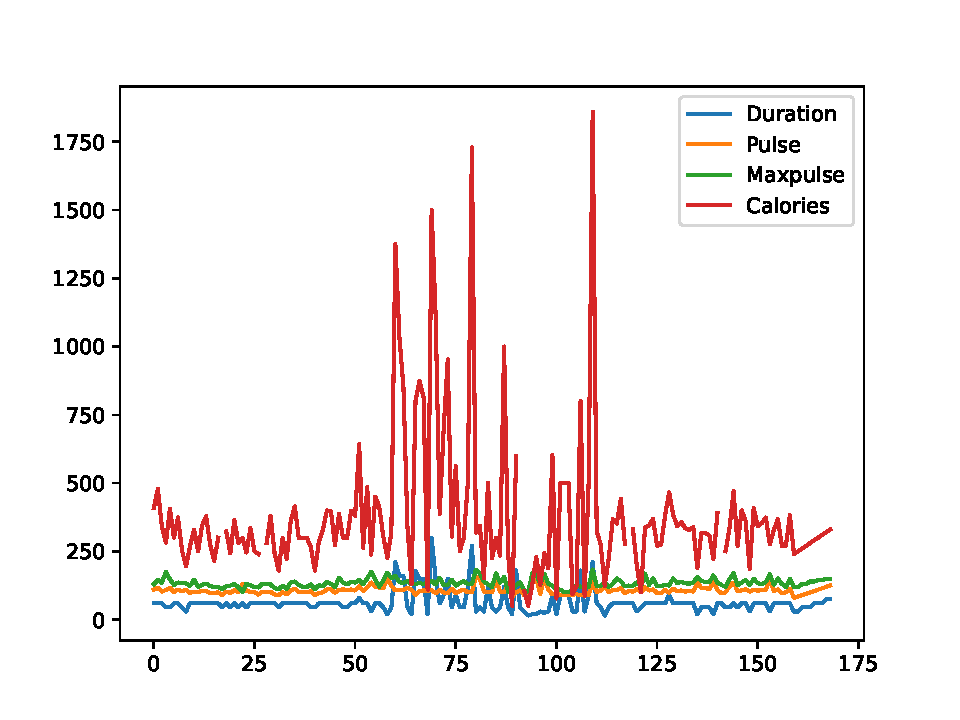
\includegraphics[scale=0.75]{img/grafica901.pdf}
  \caption{Visualización de un DataFrame}  
\end{figure}
\end{code}

\subsection{Diagrama de dispersión}

Especifique que desea un gráfico de dispersión con el argumento \texttt{kind}.
 
\begin{Shaded}
\begin{Highlighting}[]
\NormalTok{kind }\OperatorTok{=} \StringTok{\textquotesingle{}scatter\textquotesingle{}}
\end{Highlighting}
\end{Shaded}

Un diagrama de dispersión necesita un eje x y un eje y.

En el código \ref{code:dispersion}, utilizaremos ``Duración'' para el eje x y ``Calorías'' para el eje y.

Incluya los argumentos x e y de la siguiente manera:

\begin{Shaded}
  \begin{Highlighting}[]
    \NormalTok{x }\OperatorTok{=} \StringTok{\textquotesingle{}Duration\textquotesingle{}}\NormalTok{, y }\OperatorTok{=} \StringTok{\textquotesingle{}Calories\textquotesingle{}}

  \end{Highlighting}
\end{Shaded}


\begin{code} Diagrama de dispersión.

\begin{Shaded}
\begin{Highlighting}[]
\ImportTok{import}\NormalTok{ pandas }\ImportTok{as}\NormalTok{ pd}
\ImportTok{import}\NormalTok{ matplotlib.pyplot }\ImportTok{as}\NormalTok{ plt}

\NormalTok{df }\OperatorTok{=}\NormalTok{ pd.read\_csv(}\StringTok{\textquotesingle{}data/data.csv\textquotesingle{}}\NormalTok{)}

\NormalTok{df.plot(kind }\OperatorTok{=} \StringTok{\textquotesingle{}scatter\textquotesingle{}}\NormalTok{, x }\OperatorTok{=} \StringTok{\textquotesingle{}Duration\textquotesingle{}}\NormalTok{, y }\OperatorTok{=} \StringTok{\textquotesingle{}Calories\textquotesingle{}}\NormalTok{)}

\NormalTok{plt.show()}
\end{Highlighting}
\end{Shaded}

\begin{figure}[H]
  \centering
  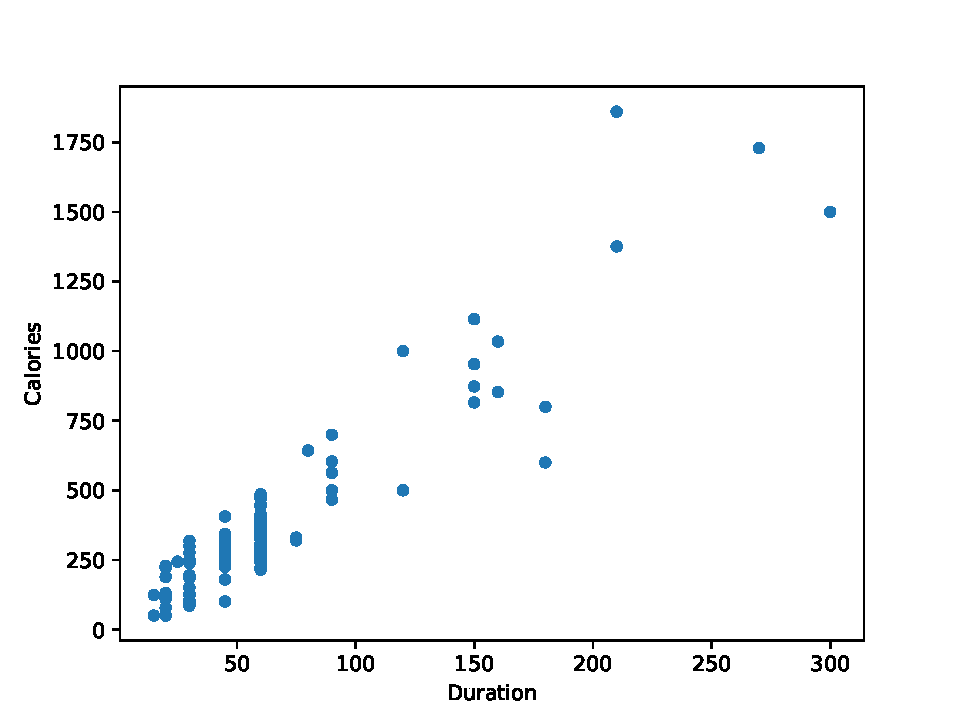
\includegraphics[scale=0.75]{img/grafica902.pdf}
  \caption{Diagrama de dispersión}
\end{figure}
\label{code:dispersion}
\end{code}
En la sección anterior, aprendimos que la correlación entre ``Duración'' y
``Calorías'' era 0.922721, y concluimos con el hecho de que una mayor
duración significa más calorías quemadas.

Al observar el diagrama de dispersión, podemos observar esa relación.

Creemos otro diagrama de dispersión, donde hay una mala relación entre
las columnas, como ``Duración'' y ``Pulso máximo'', con la correlación
0.009403.\\

\begin{code} Un diagrama de dispersión donde no hay relación entre las columnas.

\begin{Shaded}
\begin{Highlighting}[]
\ImportTok{import}\NormalTok{ pandas }\ImportTok{as}\NormalTok{ pd}
\ImportTok{import}\NormalTok{ matplotlib.pyplot }\ImportTok{as}\NormalTok{ plt}

\NormalTok{df }\OperatorTok{=}\NormalTok{ pd.read\_csv(}\StringTok{\textquotesingle{}data/data.csv\textquotesingle{}}\NormalTok{)}

\NormalTok{df.plot(kind }\OperatorTok{=} \StringTok{\textquotesingle{}scatter\textquotesingle{}}\NormalTok{, x }\OperatorTok{=} \StringTok{\textquotesingle{}Duration\textquotesingle{}}\NormalTok{, y }\OperatorTok{=} \StringTok{\textquotesingle{}Maxpulse\textquotesingle{}}\NormalTok{)}

\NormalTok{plt.show()}
\end{Highlighting}
\end{Shaded}

\begin{figure}
  \centering
  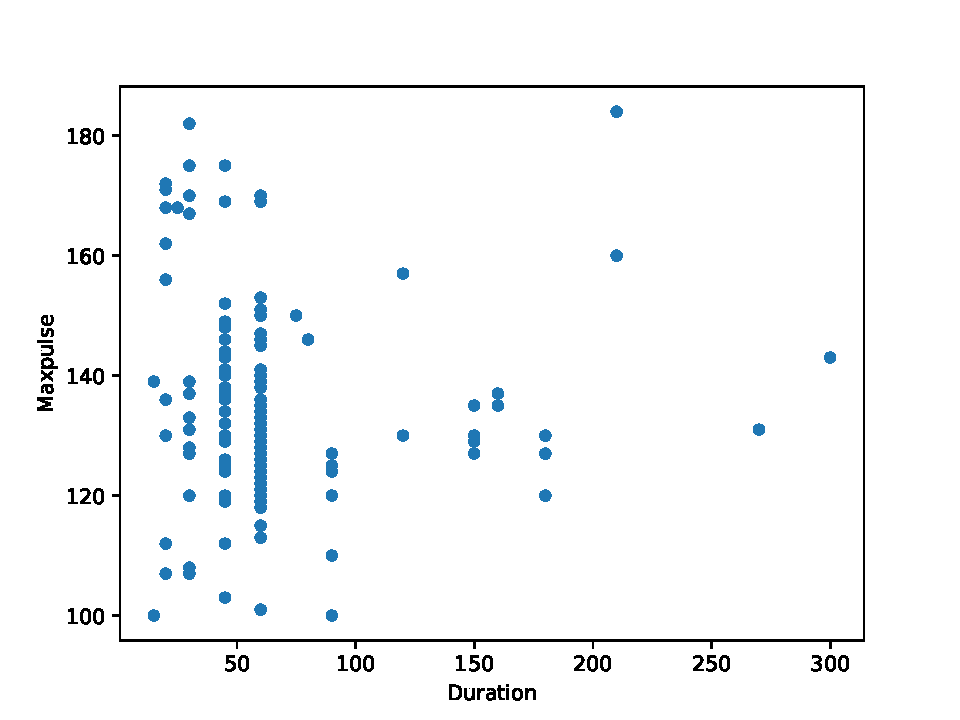
\includegraphics[scale=0.75]{img/grafica903.pdf}
  \caption{Diagrama de dispersión sin relación entre columnas}
\end{figure}
\end{code}

\subsection{Histograma}

Utilice el kindargumento para especificar que desea un histograma:
\begin{Shaded}
\begin{Highlighting}[]
\NormalTok{kind }\OperatorTok{=} \StringTok{\textquotesingle{}hist\textquotesingle{}}
\end{Highlighting}
\end{Shaded}

Un histograma solo necesita una columna. Un histograma nos muestra la
frecuencia de cada intervalo, por ejemplo ¿cuántos entrenamientos
duraron entre 50 y 60 minutos?

En el siguiente ejemplo, utilizaremos la columna "Duración" para crear
el histograma.\\

\begin{code} Histograma de un DataFrame.

\begin{Shaded}
\begin{Highlighting}[]
\NormalTok{df[}\StringTok{"Duration"}\NormalTok{].plot(kind }\OperatorTok{=} \StringTok{\textquotesingle{}hist\textquotesingle{}}\NormalTok{)}
\end{Highlighting}
\end{Shaded}

\begin{verbatim}
<Axes: ylabel='Frequency'>
\end{verbatim}

\begin{figure}
  \centering
  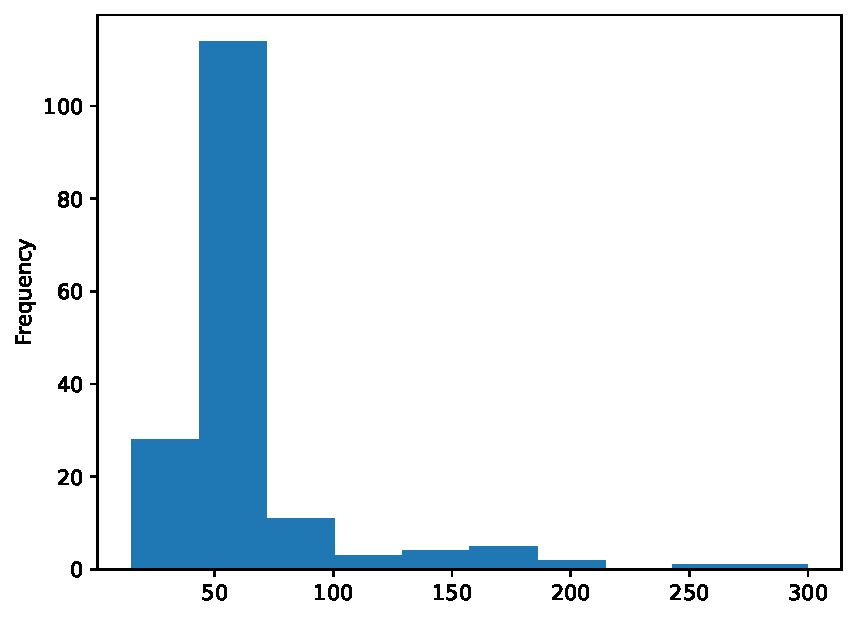
\includegraphics[scale=0.75]{img/grafica904.pdf}  
  \caption{Histograma de un DataFrame}
\end{figure}

\end{code}

El histograma nos dice que hay más de 100 ejercicios que duraron entre
50 y 60 minutos. \\

\begin{code} Ahora un histograma para las calorías.

\begin{Shaded}
\begin{Highlighting}[]
\NormalTok{df[}\StringTok{"Calories"}\NormalTok{].plot(kind }\OperatorTok{=} \StringTok{\textquotesingle{}hist\textquotesingle{}}\NormalTok{)}
\end{Highlighting}
\end{Shaded}

\begin{verbatim}
<Axes: ylabel='Frequency'>
\end{verbatim}

\begin{figure}
  \centering
  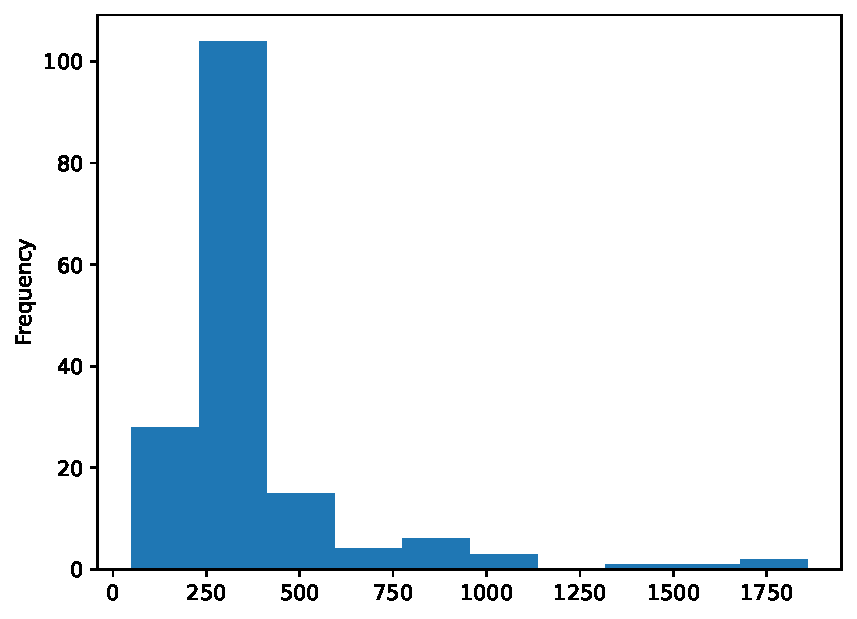
\includegraphics[scale=0.75]{img/grafica905.pdf}
  \caption{Histograma para las calorías}
\end{figure}
% \includegraphics{2c08fca6a1fb44b852da8706875c324b9e66d13e.png}
\end{code}

Este histograma nos dice que hubo poco más de 100 casos donde las
calorías quemadas fueron entre 250 y 300.

Dado que el método \texttt{plot} de Pandas utiliza \texttt{matplotlib}
como backend, si se desea modificar aspectos finos de la gráfica se debe
hacer configurando el gráfico a través de \texttt{matplotlib}
directamente.

\section{Referencias}

\begin{itemize}
  \item \href{https://www.w3schools.com/python/python_file_handling.asp}{Manejo de archivos en Python.}
  \item Lutz M., Learning Python, O\textquotesingle Reilly. 2009 
  \item \href{https://pandas.pydata.org/}{Pandas, sitio oficial.}
  \item \href{https://www.w3schools.com/python/pandas/default.asp}{Pandas en la W3Schools.}
  \item \href{https://pandas.pydata.org/docs/reference/api/pandas.DataFrame.plot.html}{Pandas Plot}
\end{itemize}
